\chapter{土の種類と含水比を用いたコーン指数の推定}
\thispagestyle{empty}
\label{ch:ConeIndexEstimation}
\minitoc

\newpage
%%%%%%%%%%%%%%%%%%%%%%%%%%%%%%%%%%%%%%%%%%%%%%%%%%%%%%%%%%%%%%%%%%%%%%%%%%%%%%%
%==============================================================================
%はじめに
%==============================================================================
\section{はじめに}
本章では,非接触での走破性判定のために本研究で提案した,スペクトル画像を用いたコーン指数推定の最後のステップである,
土の種類と含水比を用いたコーン指数推定の詳細について述べる.
本研究の提案手法において,本章で解説する部分を図\ref{fig:thesis_constitution_ch5}に茶色で示す.


まず,\ref{sec:InfluenceOfSoilTypeAndWaterContentToConeIndex}節において,
土の種類と含水比のコーン指数への影響の大きさについて解説し,
土の種類と含水比を用いてコーン指数を推定することを述べる.
% 本研究では,土の種類と含水比がコーン指数に大きく影響することを利用してコーン指数を推定する.
% 大きさではなく,関数でコーン指数を出力する先行研究の紹介でもいい?

次に,\ref{sec:ConeIndexEstimation}節において,
% \ref{sec:InfluenceOfSoilTypeAndWaterContentToConeIndex}節で述べた,
土の種類と含水比からコーン指数を推定する手法の詳細について述べる.
本研究では,マルチスペクトル画像を用いて,土の種類の識別と含水比の推定を行い,
その土の種類と含水比からコーン指数を推定することによって,非接触での走破性判定を行う.

最後に,\ref{sec:ConeindexEstimationExperiment}節において,
\ref{sec:InfluenceOfSoilTypeAndWaterContentToConeIndex}節と\ref{sec:ConeIndexEstimation}節で解説した,
コーン指数の推定手法の有効性を確認するために屋外で実施した検証実験の詳細を述べる.

\begin{figure}[p]
      \begin{center}
      \centering
      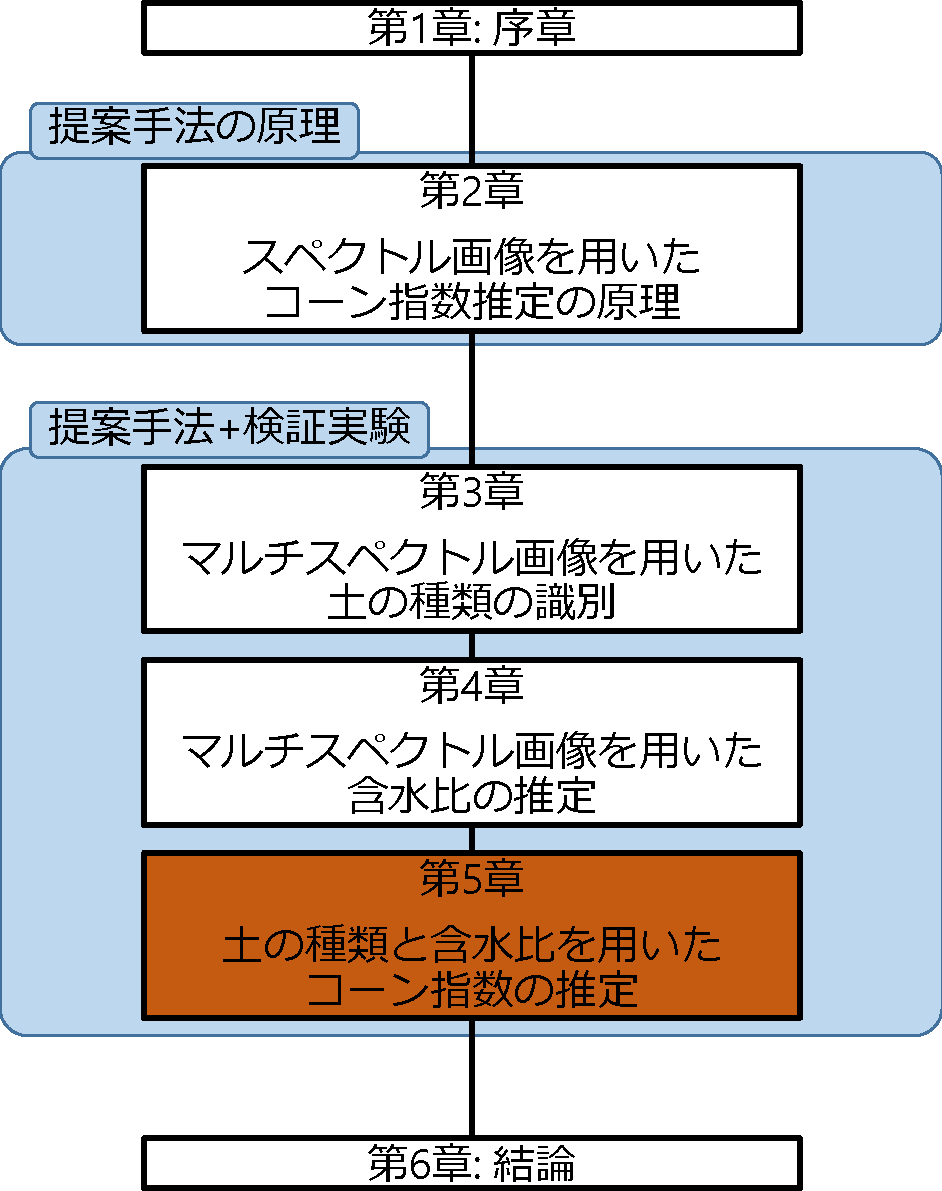
\includegraphics[width=8cm]{./Ch5_ConeIndexEstimation/Fig/thesis_constitution_ch5_compressed.pdf}
      \caption{本章で解説する部分(茶色の部分)}\label{fig:thesis_constitution_ch5}
      \end{center}
\end{figure}

\clearpage


%==============================================================================
%土の種類と含水比のコーン指数への影響
%==============================================================================
\section{土の種類と含水比のコーン指数への影響}
\label{sec:InfluenceOfSoilTypeAndWaterContentToConeIndex}

\ref{sec:PrimciplesOfConeindexEstimation}節で述べたように,土の種類と含水比はコーン指数に非常に大きな影響を与える.
従って,土の種類が,取得する波長帯の数が非常に多いマルチスペクトル画像から識別された場合,
含水比とコーン指数の関係が一意に決まる.
本研究では,これを利用することによって,マルチスペクトル画像を用いて識別した土の種類および推定した含水比からコーン指数を推定する.
コーン指数と含水比の関係の例を図\ref{fig:coneindex_and_watercontent_relationship}に示す.
この図\ref{fig:coneindex_and_watercontent_relationship}のグラフにおいては,縦軸がコーン指数,横軸が含水比を示している.
また,グラフ中にプロットされている黒いひし形が,各含水比に対するコーン指数の測定値である.
この図\ref{fig:coneindex_and_watercontent_relationship}のグラフにおいては,そのプロットされている黒いひし形の間を直線で結ぶことによって,
含水比とコーン指数の関係を表現している.
この図\ref{fig:coneindex_and_watercontent_relationship}のグラフに示すような,含水比とコーン指数の関係は,土の種類ごとに異なる.
それは,\ref{ssec:ConeindexEstimation}項における土の種類の定義より,土の種類が異なると,土の粒子の鉱物組成,有機物含有量,粒度分布,球形率が異なるため,
含水比の変動に伴うコーン指数の変動の傾向が変わるからである.
また,\ref{ssec:EstimationExperimentalProcedure}項で述べたように,
土の種類のなかでも,砂質土や礫質土と呼ばれる土が含水比に関係なく建設機械の走破に耐えうるコーン指数を維持するのに対して,粘性土と呼ばれる土は,
含水比の増加に伴って
建設機械の走破が困難になるほどコーン指数が低下することが分かっている.% 引用 4章の方に
そこで,本研究では,マルチスペクトル画像から土の種類の識別を行い,
その土の種類が粘性土であった場合には,含水比の推定を行って,
それ以外であった場合には,走破可能であると判定する.
そして,識別した土の種類と推定した含水比からコーン指数の推定を行い,
そのコーン指数を用いて走破性を判定する.

本研究においては,この含水比とコーン指数の関係を予め記録しておくことによって,
土の種類と含水比からコーン指数を推定する.
それぞれの土の種類において,含水比を変えながらコーン指数を測定することによって,
図\ref{fig:coneindex_and_watercontent_relationship}に示すような含水比とコーン指数の関係を記録する.
まず,この記録した含水比とコーン指数の関係の中から,取得する波長帯の数が非常に多いマルチスペクトル画像から土の種類を識別することによって,
コーン指数推定に用いるコーン指数と含水比の関係が分かる.
次に,ここで分かったコーン指数推定に用いるコーン指数と含水比の関係において,
推定された含水比に最も近い含水比の点を2点選び,
その2点の含水比が,推定された含水比を内分する比率$m_w:n_w$を求める.
そして,上記で選ばれた2点のコーン指数を,$m_w:n_w = m_{q_c}:n_{q_c}$となる内分比率$m_{q_c}:n_{q_c}$で内分する点から,
コーン指数の推定値を取得する.
コーン指数と含水比の関係を用いることによって推定された含水比からコーン指数の推定値を求める例を図\ref{fig:coneindex_estimation_method}に示す.
この図\ref{fig:coneindex_estimation_method}のグラフにおいて,
縦軸と横軸は,図\ref{fig:coneindex_and_watercontent_relationship}のグラフと同様に,それぞれコーン指数と含水比を示す.
また,グラフ中にプロットされている黒いひし形も,図\ref{fig:coneindex_and_watercontent_relationship}のグラフと同様に,各含水比に対するコーン指数の測定値を示す.
図\ref{fig:coneindex_estimation_method}のグラフにおいて,
コーン指数と含水比の関係を示す黒い線上にある赤い点から垂直に下におろした直線が横軸と交わる所が推定された含水比を示し,
水平に左に伸ばした直線が縦軸と交わる所がコーン指数の推定値を示す.

\begin{figure}[b]
      \begin{center}
            \begin{tabular}{c}

                  \begin{minipage}[b]{\linewidth}
                  \centering
                  \hspace{-1cm}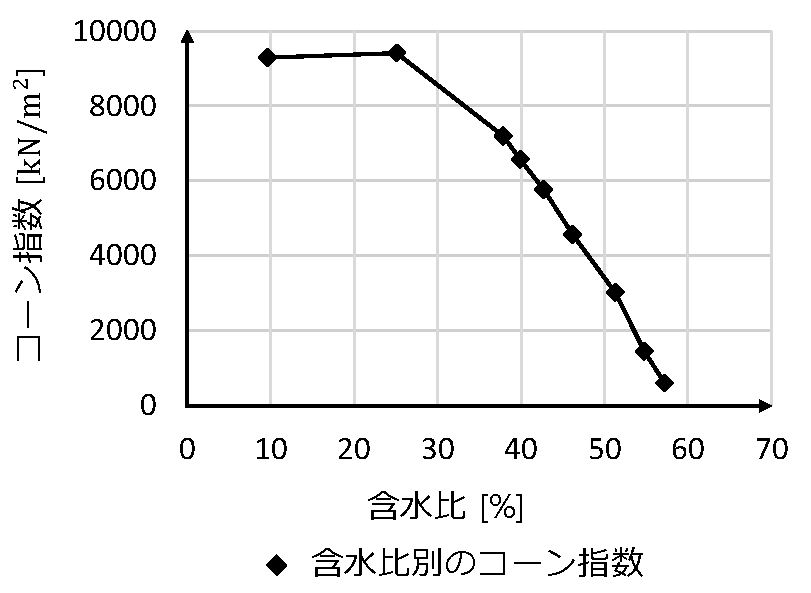
\includegraphics[width=8cm]{./Ch5_ConeIndexEstimation/Fig/coneindex_and_watercontent_relationship_compressed.pdf}
                  \caption{コーン指数と含水比の関係の例}
                  \label{fig:coneindex_and_watercontent_relationship}
                  \vspace{0.5cm}
                  \end{minipage}

                  \\

                  \begin{minipage}[b]{\linewidth}
                  \centering
                  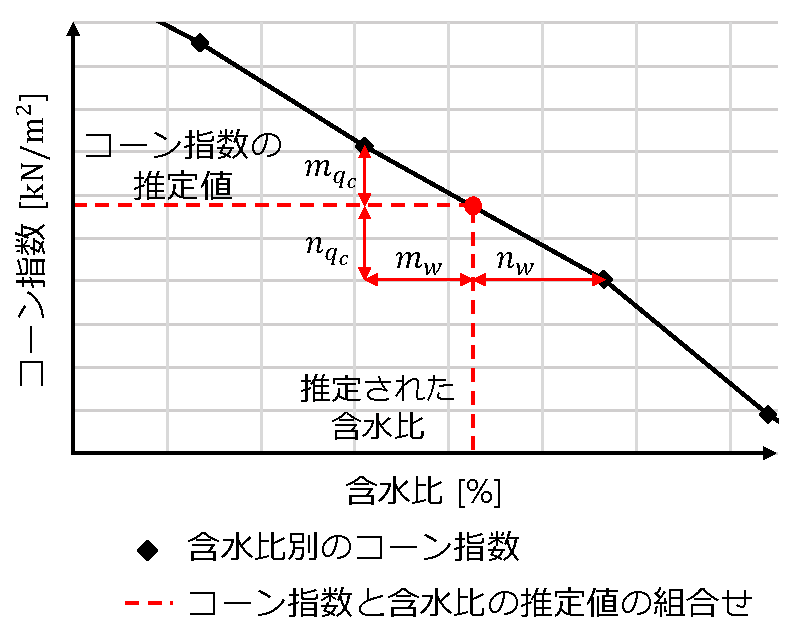
\includegraphics[width=8cm]{./Ch5_ConeIndexEstimation/Fig/coneindex_estimation_method_compressed.pdf}
                  \caption{推定された含水比からコーン指数の推定値を求める例}
                  \label{fig:coneindex_estimation_method}
                  \end{minipage}

            \end{tabular}
      \end{center}
\end{figure}

\clearpage


%==============================================================================
%含水比とコーン指数の関係の測定方法
%==============================================================================
\section{含水比とコーン指数の関係の測定方法}
\label{sec:ConeIndexEstimation}

土の種類ごとの含水比とコーン指数の関係を記録するために,複数の種類の土に対して,
含水比を変えながらコーンペネトロメータを挿入して事前にコーン指数を測定する.
% 土の種類ごとに,含水比を変えてコーン指数の値を事前に測定しておく.
コーンペネトロメータでコーン指数を測定する際には,大きな誤差が出ることが知られている.
コーンペネトロメータによって測定されるコーン指数の誤差は,
% コーン指数の測定には,
コーンペネトロメータを挿入するスピードや力の大きさ
などといった測定する人間側を原因とした誤差と,土の中にたまたま石や空洞があった場合などの
測定される土の方を原因とした誤差の2種類がある\cite{Matsuo1974}\cite{Kogure1985}.
これらの誤差を完全に除外することは困難であるが,
これらの誤差が標準正規分布に従うことは分かっている.

そこで,含水比とコーン指数の関係を記録する際には,
十分な回数の試行を実施して,
その平均値を記録した.
この図\ref{fig:coneindex_and_watercontent_relationship}のグラフ中のひし形の点としてプロットされた,
含水比ごとに測定されたコーン指数の値は,
その含水比において複数回測定した値の平均値である.
この図\ref{fig:coneindex_and_watercontent_relationship}に示したようなコーン指数と含水比の関係
を示すグラフを,土の種類と同じ数だけ記録し,
識別した土の種類と推定した含水比からコーン指数を推定する際に使用する.

\clearpage

%==============================================================================
%コーン指数推定の検証実験
%==============================================================================
\section{コーン指数推定の検証実験}
\label{sec:ConeindexEstimationExperiment}

\ref{sec:InfluenceOfSoilTypeAndWaterContentToConeIndex}節と\ref{sec:ConeIndexEstimation}節で解説した,
土の種類と含水比からコーン指数を推定する手法の有効性を確認するために,
% コーン指数推定の
検証実験を行った.

% 提案手法の,簡単な原理も含めた詳細について述べた.

% 提案手法の有効性を確認するために,
% 検証実験を行った.
取得する波長帯の数が非常に多いマルチスペクトル画像と,取得する波長帯の数が少ないマルチスペクトル画像から,
それぞれ土の種類の識別と含水比の推定を行い,その土の種類と含水比を用いたコーン指数を推定する.
それらを,実際の土の種類,測定した含水比,測定したコーン指数との間で
比較することによって,提案手法の有効性を確認した.

\subsection{実験環境}
\label{ssec:ConeindexEstimationExperimentSetting}

% 実験データについても詳細を記述

検証実験においてコーン指数推定の対象とした環境は,含水比を調整した工事現場内の屋外の土であり,
その土は,含水比が増加した場合に建設機械が走破できない程コーン指数が減少する粘性土である.
対象とする環境の様子を図\ref{fig:experimental_area}に示す.
図\ref{fig:experimental_area}の画像に示した通り,対象とする環境において,縦5m,横3mの長方形の実験場所を% "写真"ではなく"画像"とする
3カ所作り,それぞれ異なる含水比に調整して検証実験を行った.
この実験場所は,深さ0.5mまで掘削した後に,水を加えて攪拌して含水比に偏りがなくなった土で埋め戻した.
こうすることで,土の種類と含水比が均一な実験現場を作成した.
深さ0.5mまで掘削し,埋め戻す前の実験場所の画像を図\ref{fig:before_backfilled_site}に示す.
また埋め戻した後の実験場所の画像を図\ref{fig:after_backfilled_site}に示す.

\begin{figure}[b]
      \begin{center}
            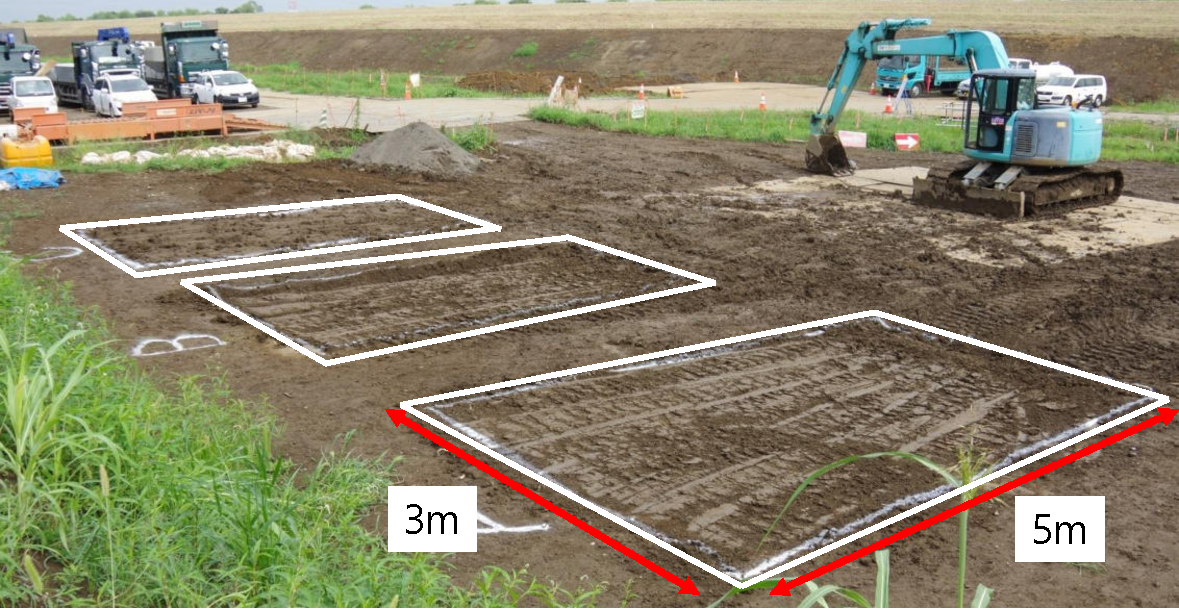
\includegraphics[width=10cm]{./Ch5_ConeIndexEstimation/Fig/experimental_area_compressed.pdf}
            \caption{検証実験の現場}
            \label{fig:experimental_area}
      \end{center}
\end{figure}

\begin{figure}[p]
      \begin{center}
            \begin{tabular}{c}

                  \begin{minipage}[b]{\linewidth}
                  \centering
                  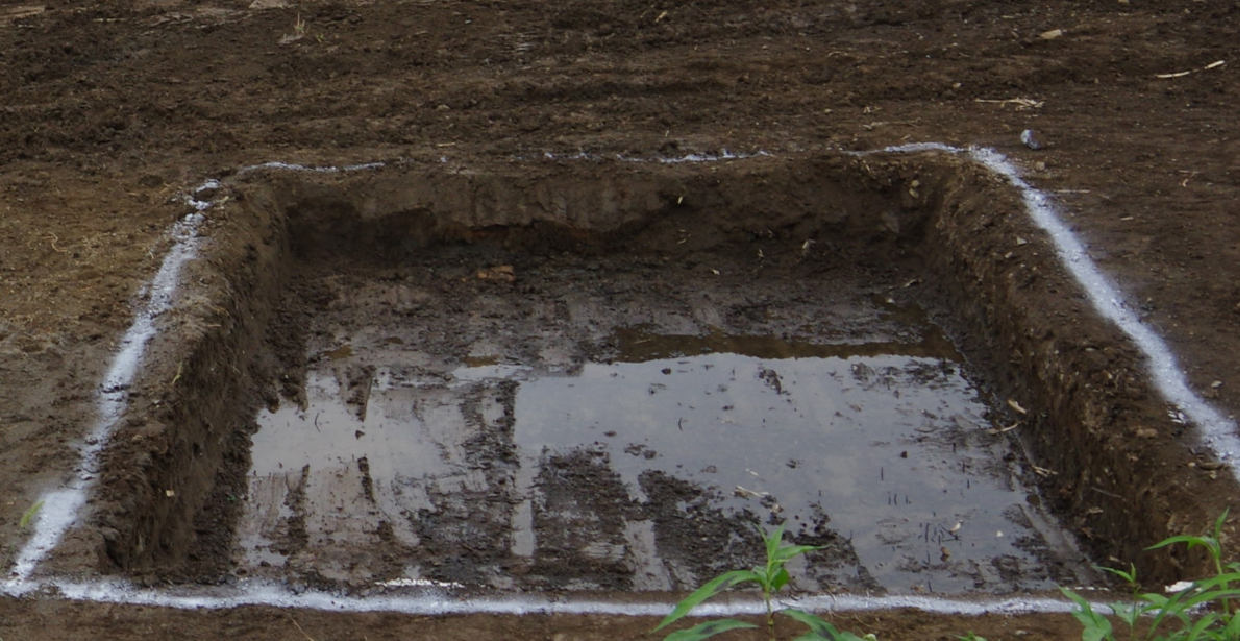
\includegraphics[width=10cm]{./ch5_ConeIndexEstimation/Fig/before_backfilled_site_compressed.pdf}
                  \caption{埋め戻す前の実験場所}\label{fig:before_backfilled_site}
                  \vspace{1cm}
                  \end{minipage}

                  \\

                  \begin{minipage}[b]{\linewidth}
                  \centering
                  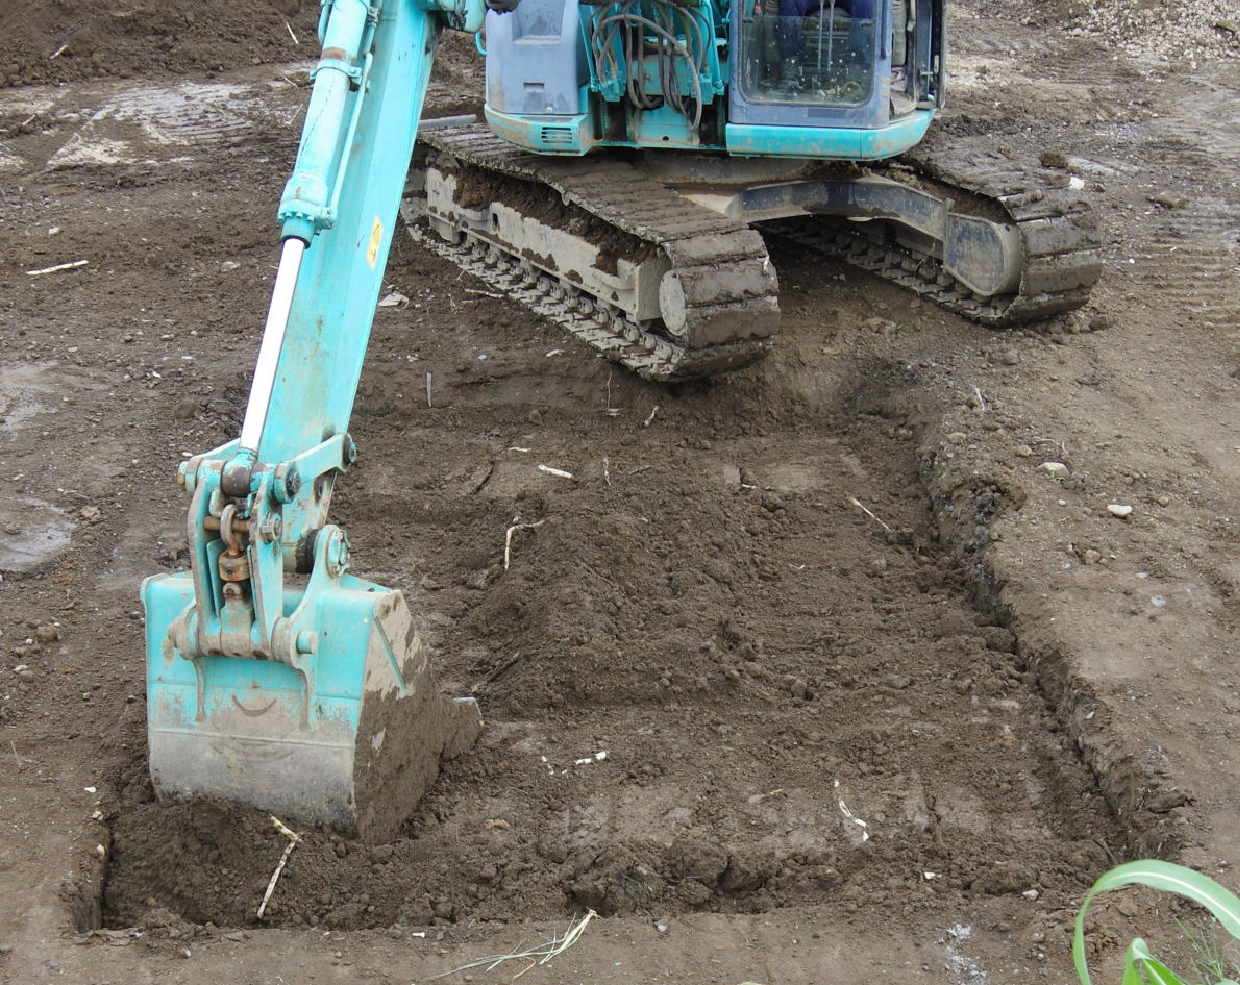
\includegraphics[width=10cm]{./ch5_ConeIndexEstimation/Fig/after_backfilled_site_compressed.pdf}
                  \caption{埋め戻した後の実験場所}\label{fig:after_backfilled_site}
                  \end{minipage}

            \end{tabular}
      % \caption{検証実験における測定の様子}\label{fig:measurement_truevalue}
      \end{center}
\end{figure}

\clearpage

本研究では,
% スペクトル画像を撮影するために,
取得する波長帯の数が非常に多いマルチスペクトル画像を撮影するためのマルチスペクトルカメラにはエヴァ・ジャパン株式会社製のNH-7を,
取得する波長帯の数が少ないマルチスペクトル画像を撮影するためのマルチスペクトルカメラにはTetracam Inc. 製のMacawを使用した.
2つのマルチスペクトルカメラの配置を,図\ref{fig:spectralcamera_arrangement}に示す.
図\ref{fig:spectralcamera_arrangement}に示した通り,2つのマルチスペクトルカメラを
建設機械の上に配置し,建設機械の進行方向にある図\ref{fig:experimental_area}で示した実験場所の粘性土を撮影した.
また,2つのマルチスペクトルカメラの画像および仕様は,
それぞれ\ref{sec:PreliminaryExperimentOfDiscrimination}節と\ref{sec:PreliminaryExperimentOfEstimation}節で示した通りである.

取得する波長帯の数が非常に多いマルチスペクトル画像と,取得する波長帯の数が少ないマルチスペクトル画像は,共に入射光を4つ以上の波長帯に分光してその光の強さを記録するため,
1つの波長帯あたりの光量が一般的なRGB画像のR, G, Bの各波長帯に
比べ少ない.
従って,一般的なRGB画像に比べてより明るい状況で撮影する必要がある.
そのため,検証実験において,マルチスペクトル画像の撮影は,
天候がよく,晴れている時に行った.
% スペクトル画像の撮影に関して,どのような条件の画像(輝度値,変動係数)を使用したのか説明?

\begin{figure}[b]
      \begin{center}
            \hspace{1.5cm}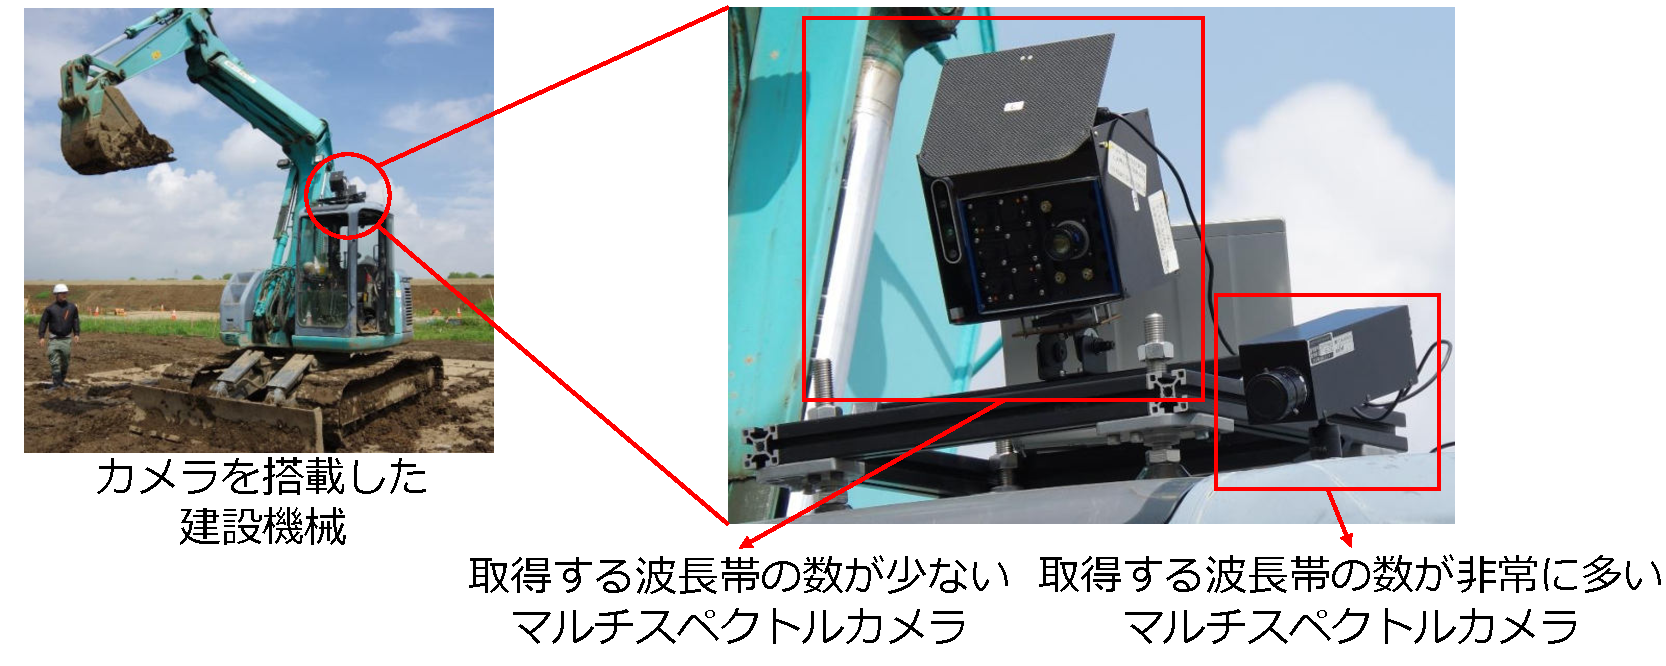
\includegraphics[width=13.5cm]{./Ch5_ConeIndexEstimation/Fig/spectralcamera_arrangement_Ver_3_compressed.pdf} % 画像が左に寄りすぎないように調整
            \caption{スペクトルカメラの配置}
            \label{fig:spectralcamera_arrangement}
      \end{center}
\end{figure}

\clearpage

% 実験データの章は不要か?

\subsection{実験手順}
\label{ssec:ConeindexEstimationExperimentProcedure}
% 下の項に合わせて,スペクトル画像の撮影と使用方法とかにでもする?

まず,異なる含水比に調整した3カ所の実験場所それぞれにおいて,
土の種類の識別と含水比の推定のために2種類のマルチスペクトルカメラを使用した.
土の種類の識別には,\ref{sec:ClassificationOfHyperspectralImage}節で解説した,
取得する波長帯の数が非常に多いマルチスペクトル画像を撮影するマルチスペクトルカメラを使用した.
一方,含水比の推定には,\ref{sec:AnalysisOfMultispectralImage}節で解説した,
取得する波長帯の数が少ないマルチスペクトル画像を撮影するマルチスペクトルカメラを使用した.
2種類のマルチスペクトルカメラを使用したのは,土の種類の識別で使用する可視光の波長と含水比の推定で使用する近赤外の波長を同時に
撮影することができないためである.
以上の2種類のマルチスペクトルカメラによる撮影の様子を,図\ref{fig:spectral_camera_shooting}に示す.
図\ref{fig:spectral_camera_shooting}の画像において,
2つのマルチスペクトルカメラを,それぞれ有線と無線で1番左に写っている
ノートPCに接続し,ノートPCで操作して撮影した.
取得する波長帯の数が非常に多いマルチスペクトル画像は,事前に撮影しておいた他の5種類の粘性土の
マルチスペクトル画像と共に学習用と評価用の画像に分け,
% 他の5種類のハイパースペクトル画像の撮影の様子も解説する? ややこしくなるからやめた方がいいかも
学習用の画像でニューラルネットワークの学習を行ったあと,評価用の画像を用いて,
$k$分割交差検証($k=5$)を行って実験場所の土の種類に対する再現率を求めた.
取得する波長帯の数が少ないマルチスペクトル画像は,水が光を吸収する近赤外の波長帯に当たる
900 $\sim$ 1700nmの波長帯の分光反射率と
水が光を吸収しない570nmの波長帯の分光反射率を取得し,
その2つの分光反射率の差から含水比を推定した.
% 含水比の推定に関して,より詳細に述べる?(フィッティングについての説明と図を追加)

次に,識別した土の種類と推定した含水比から,
予め記録していたコーン指数と含水比を参照することでコーン指数を推定した.

最後に,その実験場所において含水比とコーン指数の測定を行った.
含水比とコーン指数の測定の様子を,図\ref{fig:measurement_truevalue}に示す.

\begin{figure}[p]
      \begin{center}
            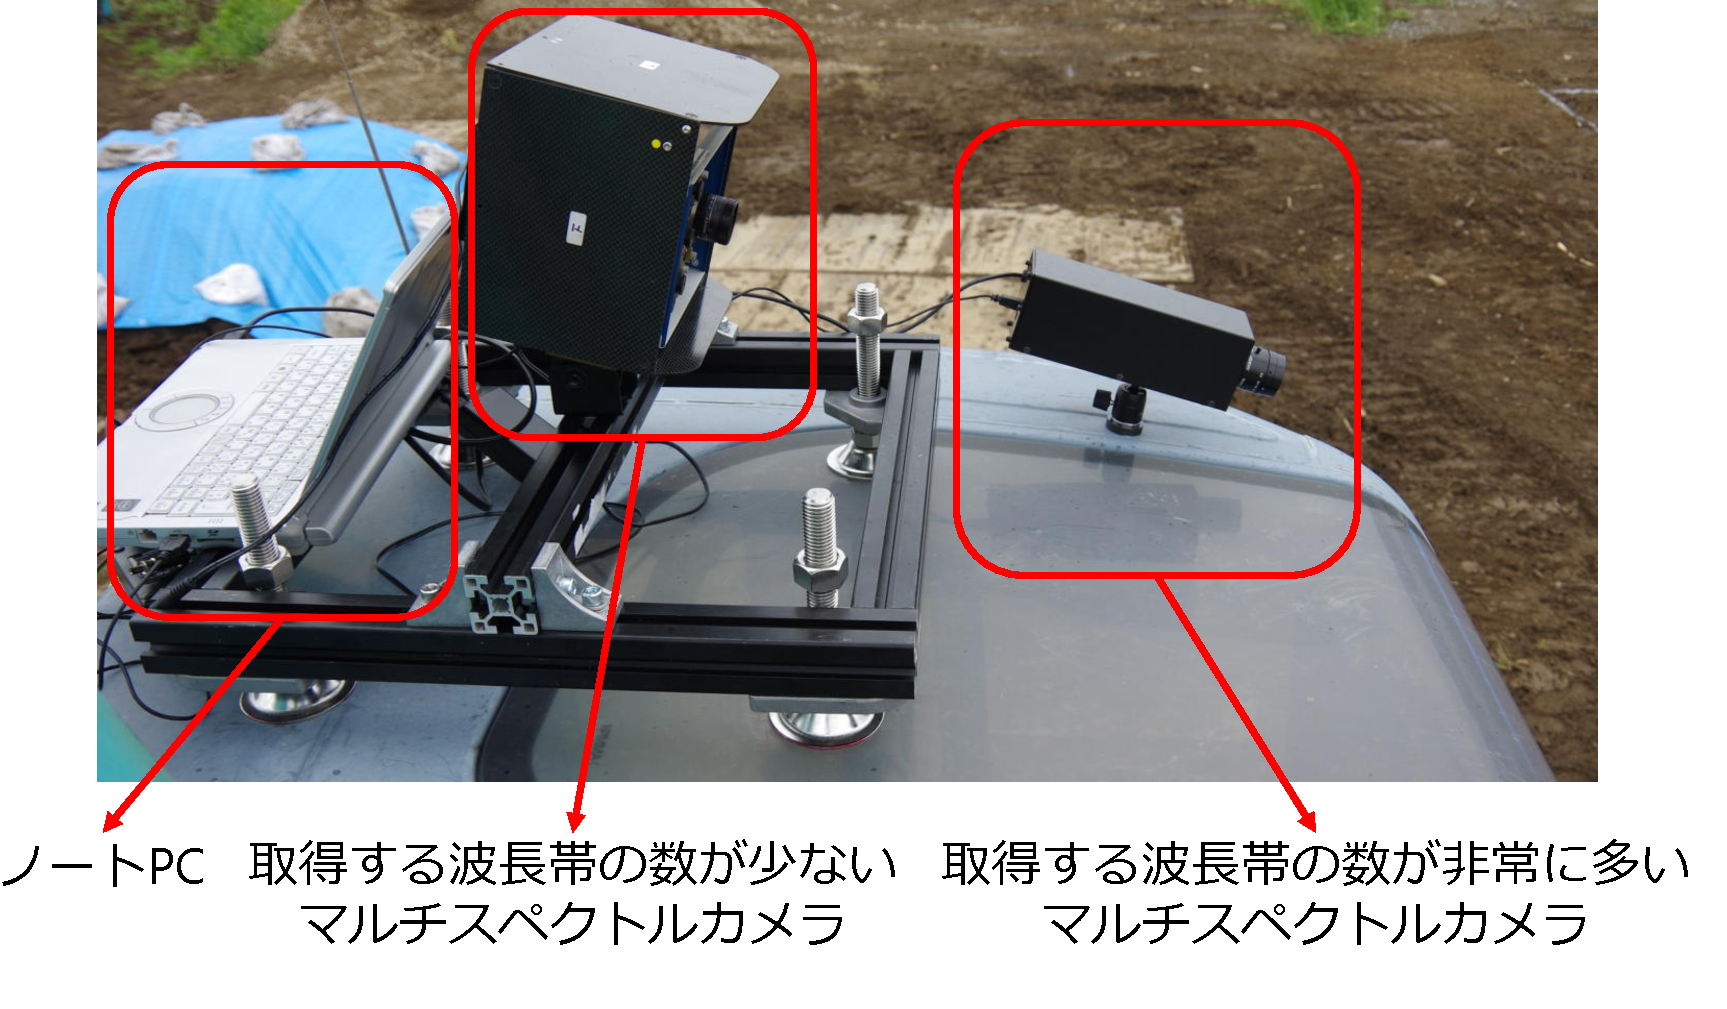
\includegraphics[width=10cm]{./Ch5_ConeIndexEstimation/Fig/spectral_camera_shooting_Ver_2_compressed.pdf}
            \caption{マルチスペクトルカメラの撮影}
            \label{fig:spectral_camera_shooting}
      \end{center}
\end{figure}


\begin{figure}[b]
      \begin{center}
            \begin{tabular}{c}

                  \begin{minipage}[b]{0.5\linewidth}
                  \centering
                  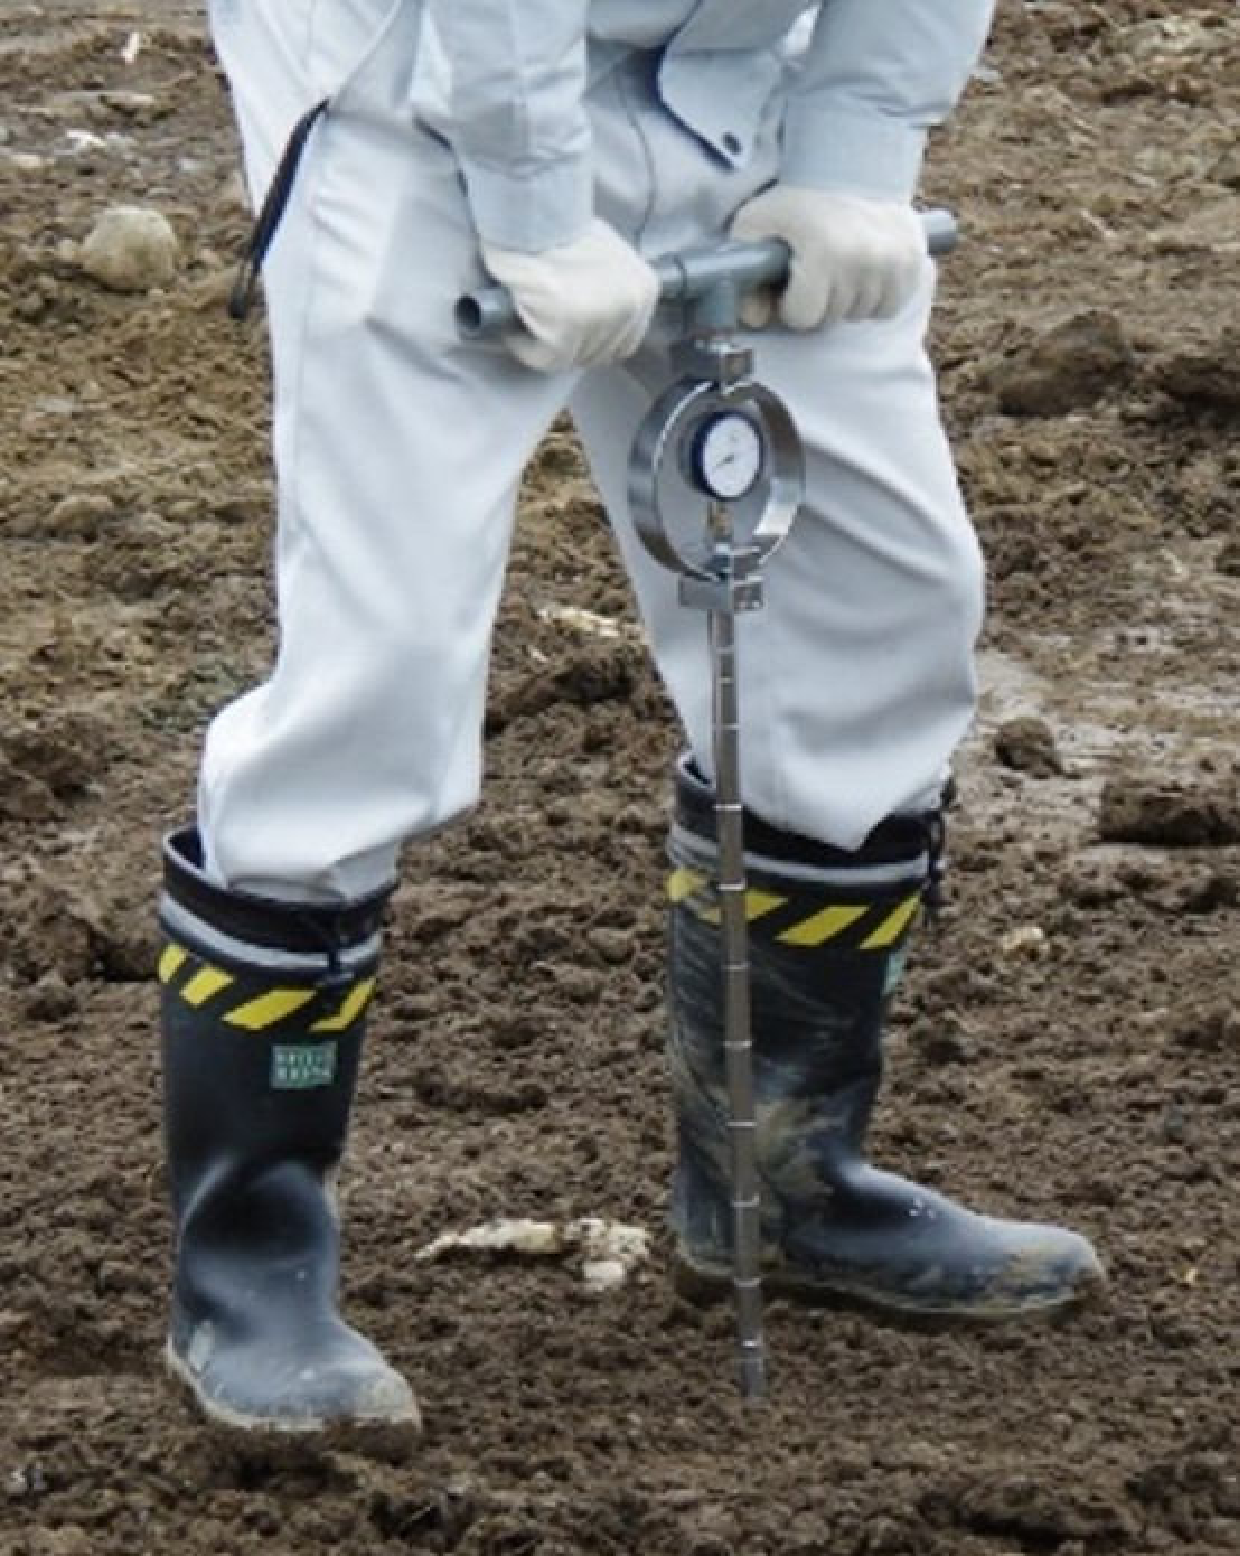
\includegraphics[height=7cm]{./ch5_ConeIndexEstimation/Fig/coneindex_measurement_compressed.pdf}
                  \caption*{(a)コーン指数の測定}
                  \end{minipage}

                  \hfill

                  \begin{minipage}[b]{0.5\linewidth}
                  \centering
                  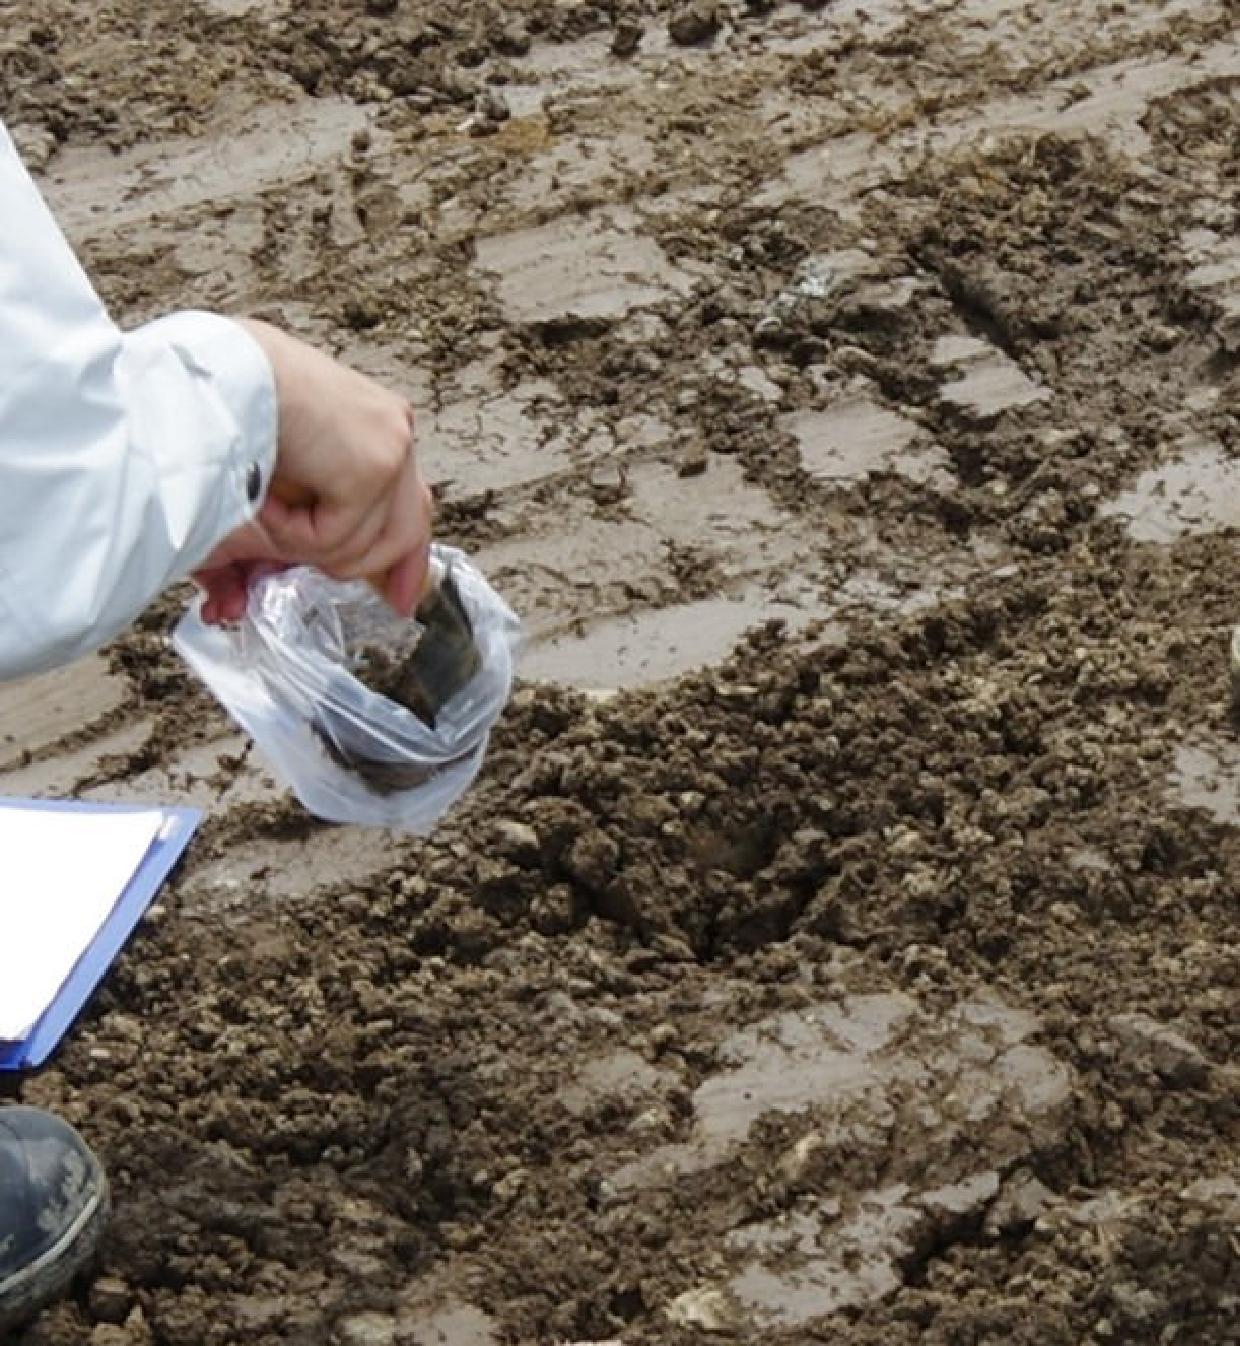
\includegraphics[height=7cm]{./ch5_ConeIndexEstimation/Fig/watercontent_measurement_compressed.pdf}
                  \caption*{(b)含水比測定に用いる土の採土}
                  \end{minipage}

            \end{tabular}
      \caption{検証実験における測定の様子}\label{fig:measurement_truevalue}
      \end{center}
\end{figure}

\clearpage


\subsection{コーン指数推定のできないマルチスペクトル画像の除外}
\label{ssec:SpectralImageCondition}

本研究では,分光反射率スペクトルを取得するために,取得する波長帯の数が非常に多いマルチスペクトル画像と,取得する波長帯の数が少ないマルチスペクトル画像を撮影するが,
適切な明るさで撮影されていないマルチスペクトル画像
からは,うまく分光反射率スペクトルを取得することができない.
そこで,撮影したマルチスペクトル画像は全て確認し,
不適切な明るさで撮影されていた画像は分光反射率スペクトルを取得する処理の対象外とした.
より詳細を述べると,取得する波長帯の数が非常に多いマルチスペクトル画像については,画素ごとに明るさを確認した.
各画素に対して,350 $\sim$ 450nmの波長帯の光の強さの平均と,700 $\sim$ 750nmの光の強さの平均を比較し,
\begin{eqnarray}
(350 \sim 450{\rm nm}の波長帯の光の強さの平均) \times 10 > \nonumber\\ (700 \sim 750{\rm nm}の光の強さの平均),\label{eq:reflectance_spectrum}
\end{eqnarray}
である場合には,その画素は土粒子の影になって土粒子の分光反射率スペクトルを取得できていないと判定し,
分光反射率スペクトルを取得する処理の対象外とした.
土粒子の影になっている部分の分光反射率スペクトルと土粒子の分光反射率スペクトルを比較した例を図\ref{fig:hyperspectral_image_selection}に示す.
まず,図\ref{fig:hyperspectral_image_selection}の左側の画像はマルチスペクトル画像の生画像である.黄色い枠に囲まれた部分が土粒子の影になっている部分であり,
濃い青の枠で囲まれた部分が影になっていない部分である.次に,図\ref{fig:hyperspectral_image_selection}の右側のグラフにおいて,黄色い線は,左側の画像において
黄色い枠で囲まれた部分の分光反射率スペクトルの平均を示し,濃い青の線は,左側の画像において濃い青の枠で囲まれた部分の分光反射率スペクトルの平均を示す.
図\ref{fig:hyperspectral_image_selection}の右側のグラフより,
土粒子の影になっている部分の分光反射率スペクトルは,土粒子の部分の分光反射率スペクトルに比べ,扁平になっているのが分かる.
本研究で撮影した取得する波長帯の数が非常に多いマルチスペクトル画像の各画素において,この黄色い線のような扁平な分光反射率スペクトルは,式(\ref{eq:reflectance_spectrum})に基づいて,土粒子の分光反射率スペクトルを
表していないと判定し,処理の対象外とした.

一方,取得する波長帯の数が少ないマルチスペクトル画像については,画像自体の明るさと,
検証実験を実施した工事現場内に設置した,分光反射率スペクトルが既知の校正シートの輝度値の分散の程度を確認した.
画像自体の明るさに関しては,本研究で使用したTetracam Inc. 製のMacawで撮影したマルチスペクトル画像の輝度値を確認した.
画像の中で校正シートと実験場所を示す部分の輝度値の平均がMacawで取りうる輝度値の最大値に対して7.62\% $\sim$ 91.6\%に
収まらなかった画像を,校正シートと実験場所の土の分光反射率を取得できていないと判定し,
分光反射率を取得する処理の対象外とした.
暗すぎるマルチスペクトル画像と明るすぎるマルチスペクトル画像の例を,それぞれ図\ref{fig:inappropriate_brightness_multispectral_image}(a)および(b)に示す.図\ref{fig:inappropriate_brightness_multispectral_image}(a)および(b)より,
不適切な明るさの画像からは適切な分光反射率を取得することは困難であることが分かる.
一方,適切な明るさのマルチスペクトル画像の例を図\ref{fig:appropriate_brightness_multispectral_image}に示す.
本研究では,図\ref{fig:appropriate_brightness_multispectral_image}に示すようなマルチスペクトル画像から分光反射率スペクトルを取得した.
また,校正シートの輝度値の分散の程度に関しては,校正シートを撮影した部分の輝度値の変動係数を確認した.
変動係数が0.05以上である場合は,校正シートの適切な分光反射率を取得できていないと判定して,
分光反射率を取得する処理の対象外とした.
校正シートの反射光が取得できていない画像と
校正シートの反射光が取得できた画像を,それぞれ図\ref{fig:inappropriate_dispersion_calibration_panel}(a)および(b)に示す.
図\ref{fig:inappropriate_dispersion_calibration_panel}(a)の左側にある輝度値の分布を示すグラフにおいては,
輝度値のピークがいくつも立っており,単一の物質である校正シートの反射光以外の光も一緒に入ってきていることが分かる.
図\ref{fig:inappropriate_dispersion_calibration_panel}(a)の右側にある画像を見ると,校正シートのすぐそばに
草が生えていることが分かる.この草が太陽光を反射して2次光源となったため,輝度値のピークがいくつも立っている.
一方,図\ref{fig:inappropriate_dispersion_calibration_panel}(b)の左側にある輝度値の分布を示すグラフにおいては,
輝度値のピークが1つであることが分かる.この輝度値の変動係数は0.05未満であるため,校正シートの反射光のみが入射してきていると判定している.

以上で解説した手法で不適切な画像を除外し,除外していない画像から分光反射率スペクトルを取得する.

\begin{figure}[b]
      \begin{center}
            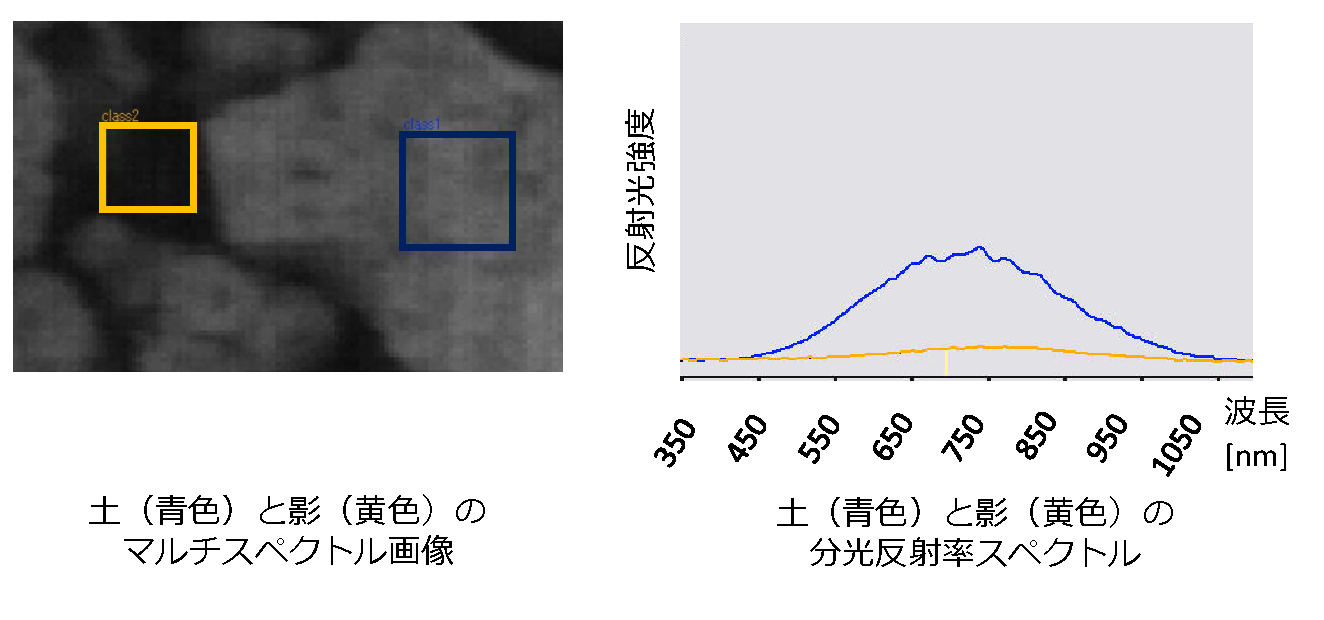
\includegraphics[width=11cm]{./Ch5_ConeIndexEstimation/Fig/hyperspectral_image_selection_compressed.pdf}
            \caption{マルチスペクトル画像の画素の選別}
            \label{fig:hyperspectral_image_selection}
      \end{center}
\end{figure}

\clearpage

\begin{figure}[p]
      \begin{center}
            \begin{tabular}{c}

                  \begin{minipage}[b]{\linewidth}
                  \centering
                  \includegraphics[height=4cm]{./ch5_ConeIndexEstimation/Fig/too_dark_multispectral_image_compressed.pdf}
                  \caption*{(a)暗すぎる画像}
                  \end{minipage}

                  \\

                  \begin{minipage}[b]{\linewidth}
                  \centering
                  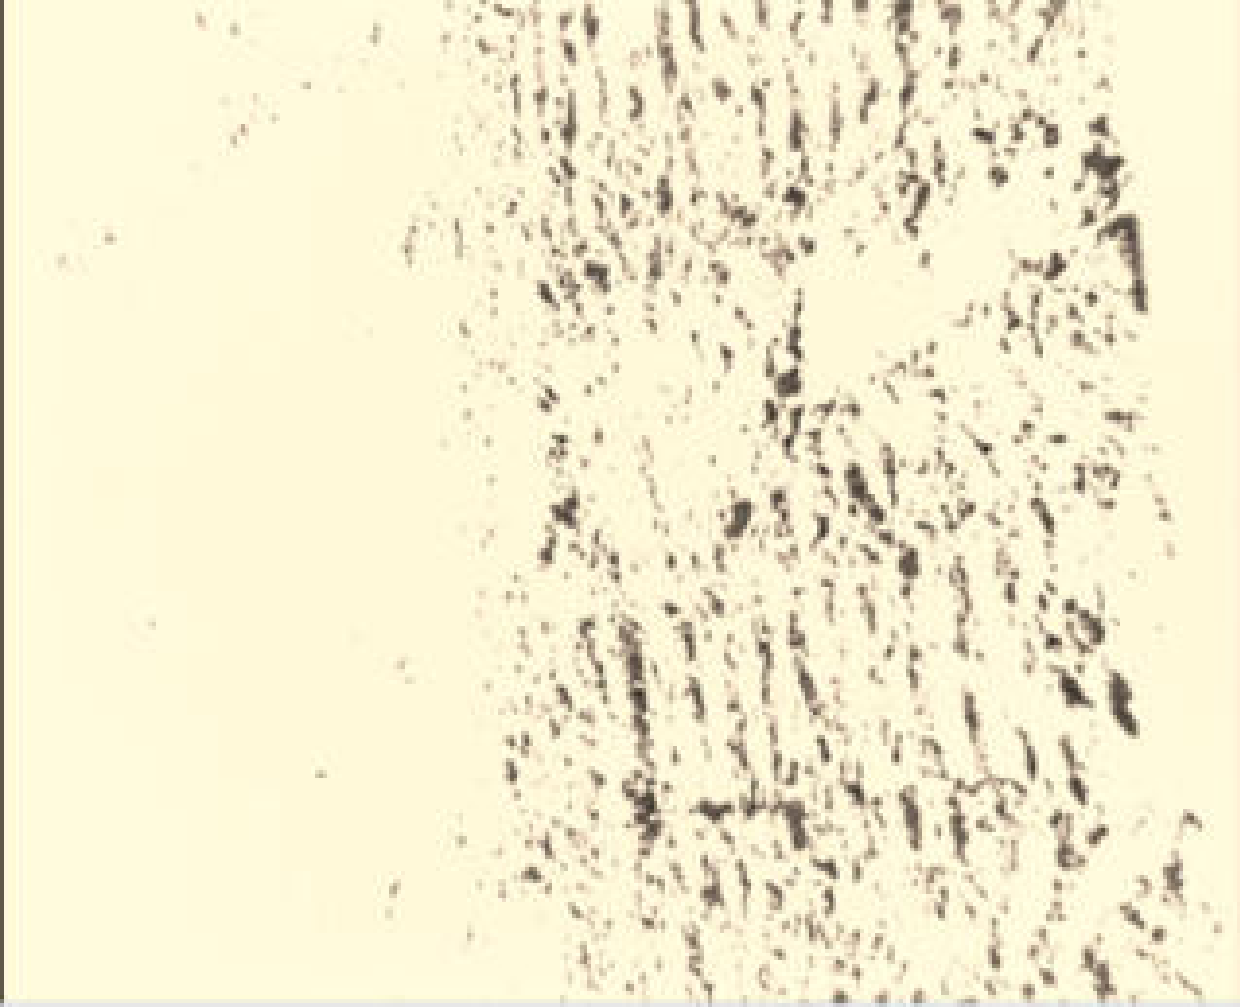
\includegraphics[height=4cm]{./ch5_ConeIndexEstimation/Fig/too_bright_multispectral_image_compressed.pdf}
                  \caption*{(b)明るすぎる画像}
                  \end{minipage}

            \end{tabular}
      \caption{不適切な明るさのマルチスペクトル画像}\label{fig:inappropriate_brightness_multispectral_image}
      \end{center}
\end{figure}

\begin{figure}[p]
      \begin{center}
            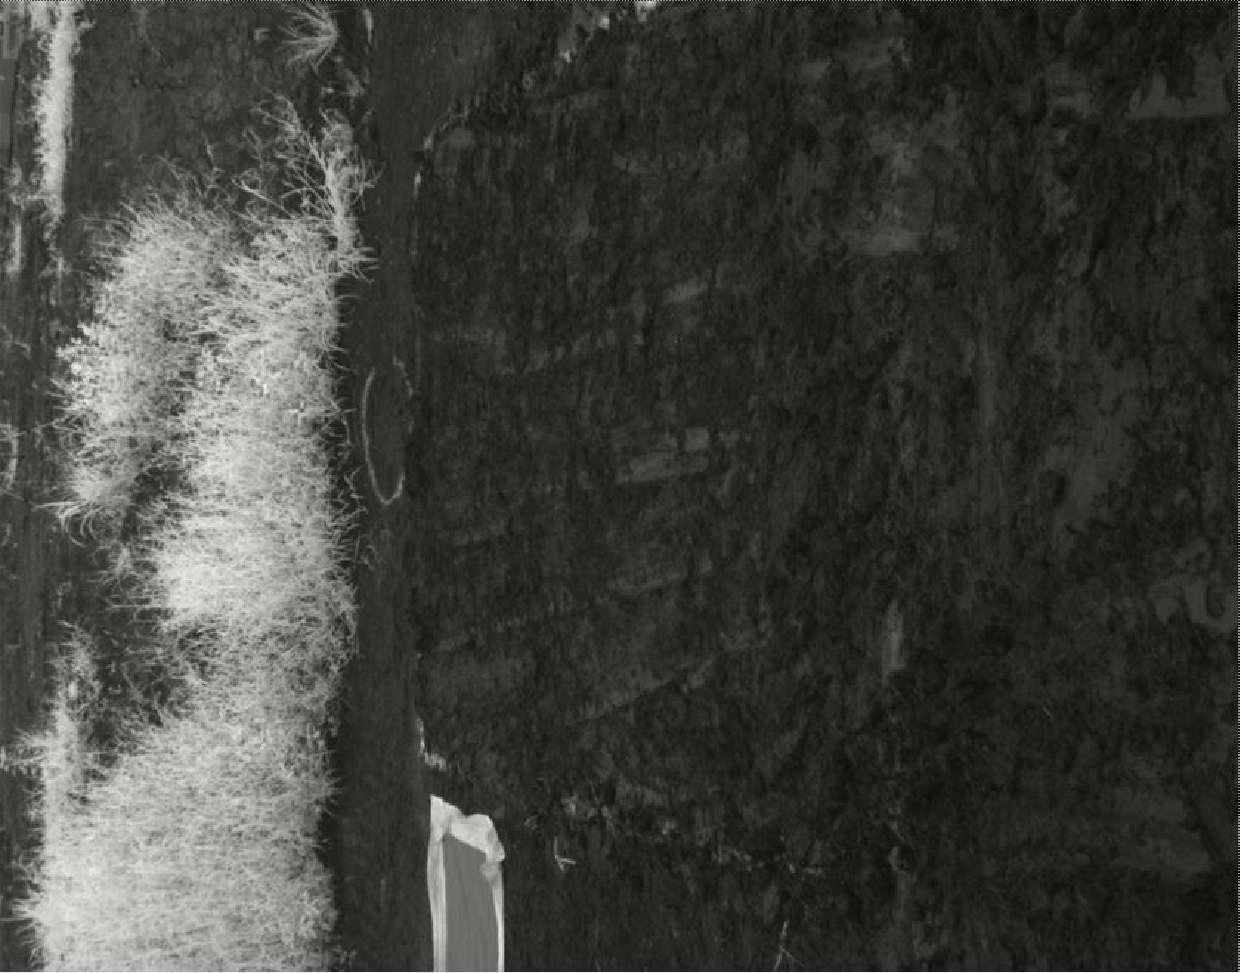
\includegraphics[height=4cm]{./Ch5_ConeIndexEstimation/Fig/appropriate_brightness_multispectral_image_compressed.pdf}
            \caption{適切な明るさのマルチスペクトル画像}
            \label{fig:appropriate_brightness_multispectral_image}
      \end{center}
\end{figure}

\clearpage

\begin{figure}[p]
      \begin{center}
            \begin{tabular}{c}

                  \begin{minipage}[b]{\linewidth}
                  \centering
                  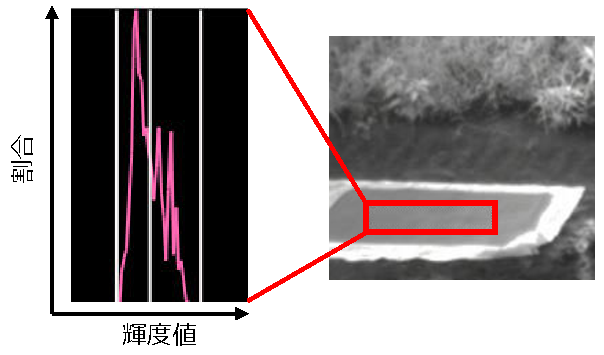
\includegraphics[height=4.5cm]{./ch5_ConeIndexEstimation/Fig/too_large_dispersion_calibration_panel_compressed.pdf}
                  \caption*{(a)校正シートの反射光が取得できていない例}
                  \vspace{1cm}
                  \end{minipage}

                  \\

                  \begin{minipage}[b]{\linewidth}
                  \centering
                  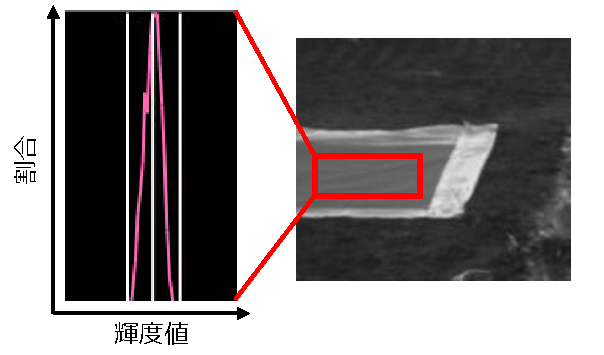
\includegraphics[height=4.5cm]{./ch5_ConeIndexEstimation/Fig/too_small_dispersion_calibration_panel_compressed.pdf}
                  \caption*{(b)校正シートの反射光が取得できている例}
                  \end{minipage}

            \end{tabular}
      \caption{校正シートの反射光}\label{fig:inappropriate_dispersion_calibration_panel}
      \end{center}
\end{figure}

\clearpage

\subsection{実験結果}
\label{ssec:ConeindexEstimationExperimentResult}

まず,実験現場の粘性土を含めた6種類の粘性土の土を,取得する波長帯の数が非常に多いマルチスペクトル画像から取得した分光反射率スペクトルで識別した結果の
混同行列を図\ref{fig:coneindex_estimation_confusion_matrix}に示す.
この検証実験では,\ref{ssec:NeuralNetWork}項で解説したニューラルネットワークを用いて,
バッチサイズを128,エポック数を12に設定して学習を行い,6種類の粘性土のマルチスペクトル画像から
土の種類を識別した.
識別の結果として得られた図\ref{fig:coneindex_estimation_confusion_matrix}の混同行列において,
縦軸は取得した分光反射率スペクトルが撮影された本当の土の種類を示し,横軸は\ref{ssec:NeuralNetWork}項で解説したニューラルネットワークによって識別された土の種類を示す.
また,この混同行列においては,青い色が濃くなるほど確率が高くなる.
本当の土の種類とニューラルネットワークによって識別された土の種類が一致した場合,混同行列の対角成分の確率がそれ以外の成分の確率に比べ高くなる.
図\ref{fig:coneindex_estimation_confusion_matrix}の混同行列より,本当の土の種類と識別された土の種類が高い確率で一致したことが分かった.
さらに,実験現場で撮影したマルチスペクトル画像から取得した分光反射率スペクトルを,97.7\%の再現率で識別できた.
これらのことから,マルチスペクトル画像を用いて波長分解能の高い分光反射率スペクトルを取得することにより,
土の種類を識別できることが分かった.

\begin{figure}[b]
      \begin{center}
            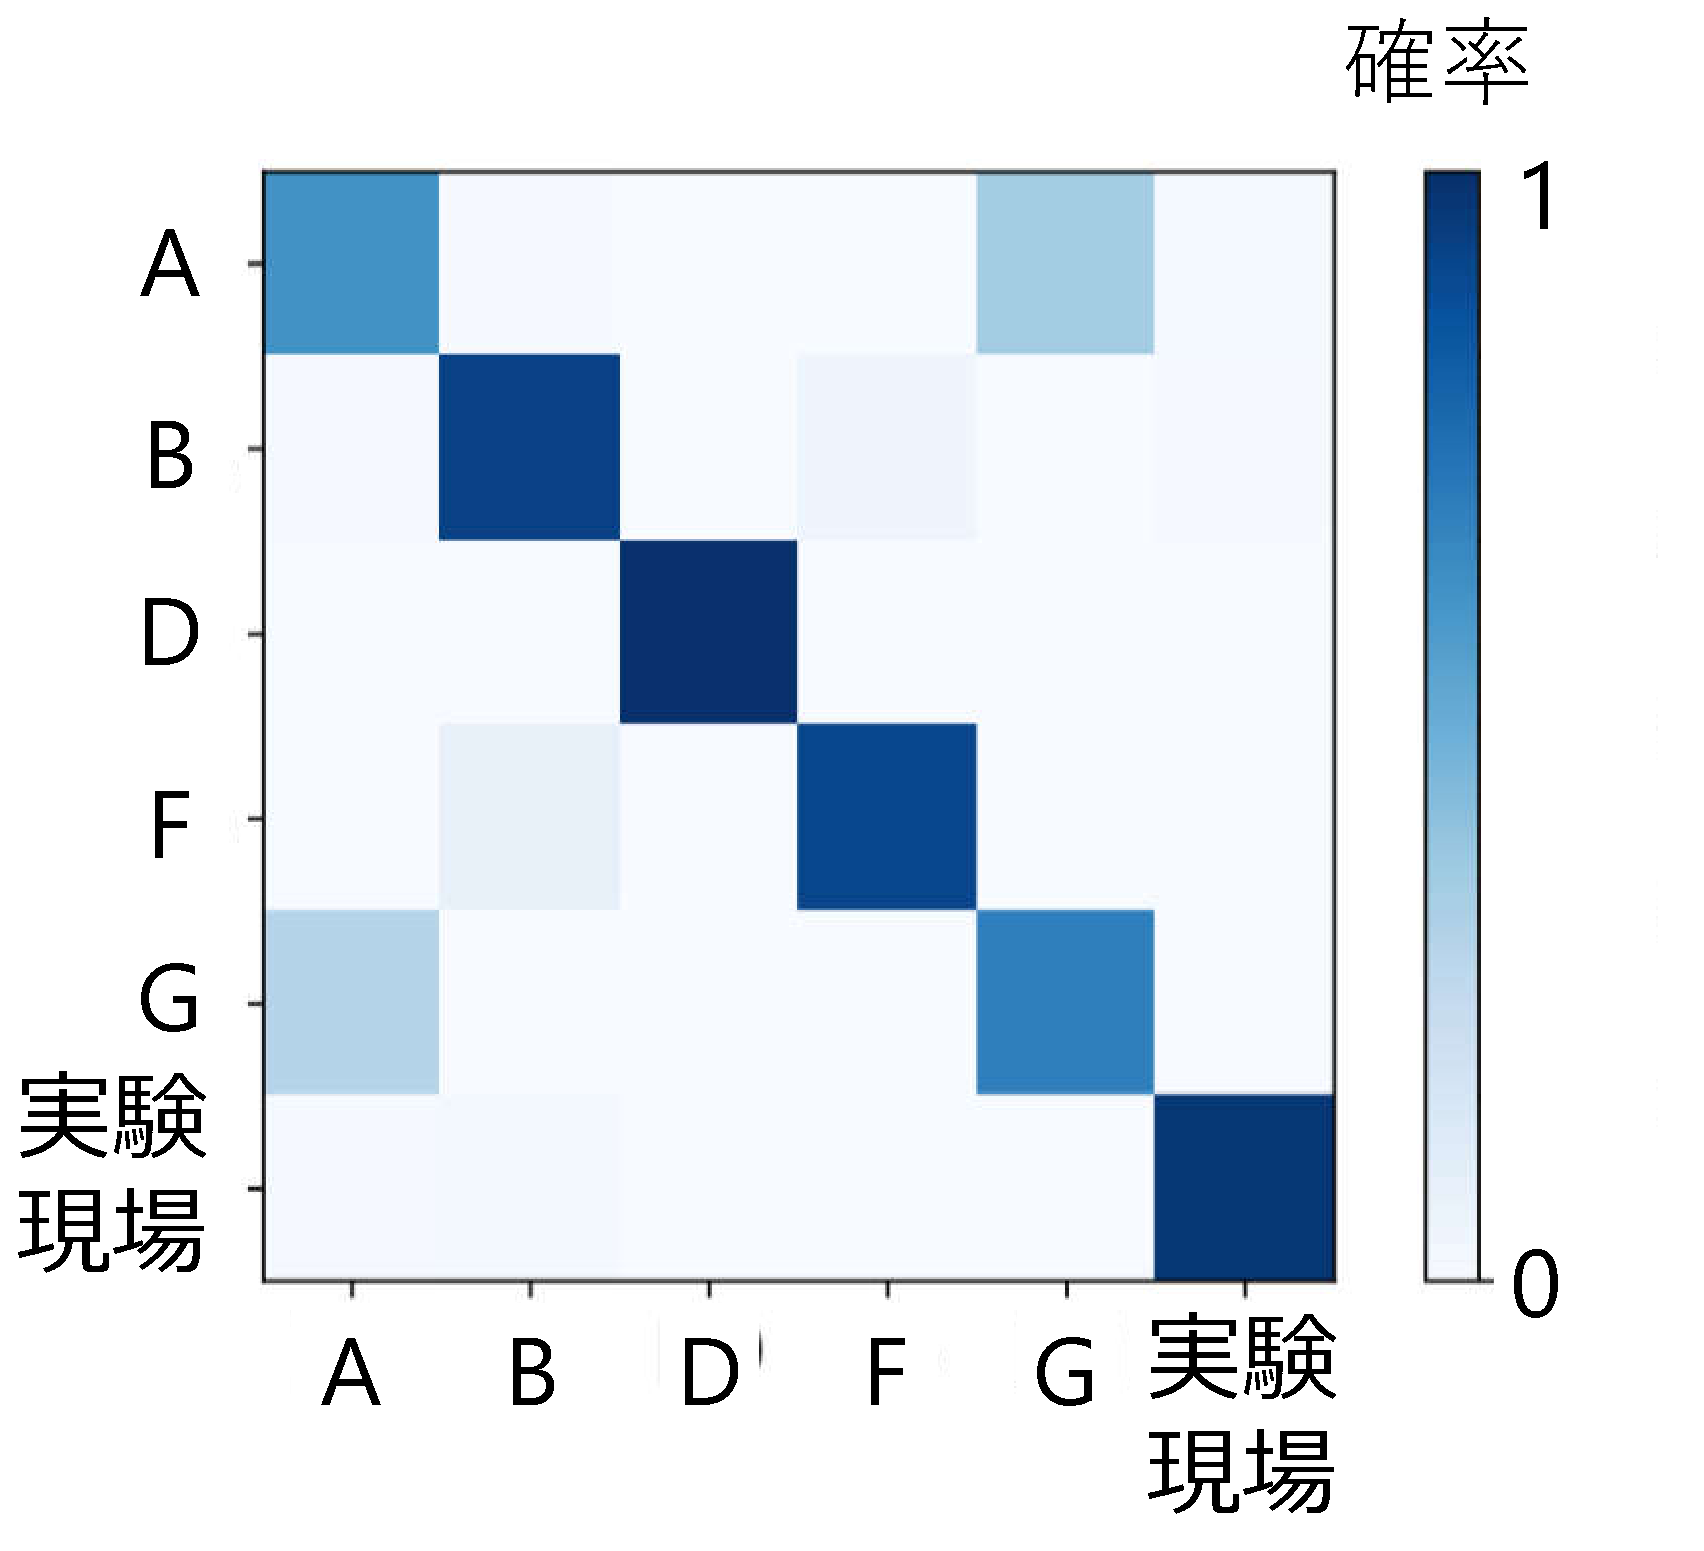
\includegraphics[width=6cm]{./ch5_ConeIndexEstimation/Fig/coneindex_estimation_confusion_matrix_compressed.pdf}
            \caption{6種類の粘性土の識別結果を示す混同行列}
            \label{fig:coneindex_estimation_confusion_matrix}
      \end{center}
\end{figure}

\clearpage

次に,含水比とコーン指数の,実験場所で測定した実測値,提案手法で推定した推定値,実測値と推定値の誤差の絶対値の3つの値を
表\ref{table.Calculated_cone_index}に示す.
この表\ref{table.Calculated_cone_index}において,含水比の誤差は3つとも大きくなく,含水比が精度 
良く推定できていることが分かる.一方,コーン指数の誤差については,表\ref{table.Calculated_cone_index}の上から2番目 
と3番目は精度良く推定できているが,1番上の誤差が大きい.
これは,検証実験の対象となった土の含水比とコーン指数の関係が原因である.
この検証実験の対象となった,含水比を調整した工事現場内の屋外の土の,含水比とコーン指数の関係を図\ref{fig:coneindex_and_watercontent_relationship_of_experimental_site}に示す.
図\ref{fig:coneindex_and_watercontent_relationship_of_experimental_site}のグラフにおいて,
縦軸はコーン指数,横軸は含水比を示し,黒いひし形は含水比別のコーン指数を示す.
ここで解説するコーン指数推定の検証実験においては,この図\ref{fig:coneindex_and_watercontent_relationship_of_experimental_site}のグラフに
基づいて,推定した含水比からコーン指数を推定する.

表\ref{table.Calculated_cone_index}の上から2番目 
と3番目の,コーン指数の推定精度が高い場合は,図\ref{fig:coneindex_and_watercontent_relationship_of_experimental_site}のグラフに示す通り含水比の実測値と推定値の存在する45\%から49\%の間で
コーン指数の変動が小さいため,含水比の誤差が数\%程度ではコーン指数の誤差は非常に小さい.
表\ref{table.Calculated_cone_index}の上から2番目 
と3番目における,コーン指数と含水比の実測値および推定値の組合せを,それぞれ図\ref{fig:validationsoil_coneindex_and_watercontent_relationship_2ndrow_and_3rdrow}(a)および(b)に示す.
図\ref{fig:validationsoil_coneindex_and_watercontent_relationship_2ndrow_and_3rdrow}(a)および(b)のグラフにおいて,
縦軸はコーン指数,横軸は含水比を示す.
また,黒いひし形は,図\ref{fig:coneindex_and_watercontent_relationship_of_experimental_site}のグラフにおける
黒いひし形と同様に含水比別のコーン指数を示し,青い実線と赤い点線は,それぞれコーン指数と含水比の実測値の組合せ,およびコーン指数と含水比の推定値の組合せを示す.
図\ref{fig:validationsoil_coneindex_and_watercontent_relationship_2ndrow_and_3rdrow}(a)では,
表\ref{table.Calculated_cone_index}の上から2番目におけるコーン指数と含水比の実測値および推定値の組合せを示し,
図\ref{fig:validationsoil_coneindex_and_watercontent_relationship_2ndrow_and_3rdrow}(b)では,
表\ref{table.Calculated_cone_index}の上から3番目におけるコーン指数と含水比の実測値および推定値の組合せを示す.
図\ref{fig:validationsoil_coneindex_and_watercontent_relationship_2ndrow_and_3rdrow}(a)および(b)のグラフにおける,
実測値,推定値,誤差は,それぞれ表\ref{table.Calculated_cone_index}におけるコーン指数の実測値,推定値,誤差の値と対応している.
図\ref{fig:validationsoil_coneindex_and_watercontent_relationship_2ndrow_and_3rdrow}(a)及び(b)に示す通り,
含水比の実測値と推定値の存在する45\%から49\%の間でコーン指数の変動が小さいために,
コーン指数の実測値と推定値を示す水平方向の青い実線と赤い点線がほぼ重なっており,
コーン指数の誤差が非常に小さいことが分かる.

一方,表\ref{table.Calculated_cone_index}の1番上の,コーン指数の推定精度が低い場合は,図\ref{fig:coneindex_and_watercontent_relationship_of_experimental_site}のグラフに示す通り含水比の実測値と推定値の存在する38\%から42\%の間でコーン指数が大きく減少し,含水比に対するコーン指数の変動が大きいため,含水比の誤差が数\%程度でもコーン指数の誤差は非常に大きい.
表\ref{table.Calculated_cone_index}の1番上における,コーン指数と含水比の実測値および推定値の組合せを,
図\ref{fig:validationsoil_coneindex_and_watercontent_relationship}に示す.
図\ref{fig:validationsoil_coneindex_and_watercontent_relationship}のグラフにおいて,
縦軸と横軸は,図\ref{fig:validationsoil_coneindex_and_watercontent_relationship_2ndrow_and_3rdrow}(a)および(b)のグラフと同様に,
コーン指数と含水比を示す.
また,黒いひし形は図\ref{fig:coneindex_and_watercontent_relationship_of_experimental_site}のグラフと同様に含水比別のコーン指数を示し,
青い実線と赤い点線は,それぞれコーン指数と含水比の実測値の組合せ,コーン指数と含水比の推定値の組合せを示す.
さらに,図\ref{fig:validationsoil_coneindex_and_watercontent_relationship}のグラフにおける実測値,推定値,誤差は,それぞれ表\ref{table.Calculated_cone_index}におけるコーン指数の実測値,推定値,誤差を示す.
図\ref{fig:validationsoil_coneindex_and_watercontent_relationship}に示す通り,
含水比の実測値と推定値の存在する38\%から42\%の間でコーン指数の変動が大きいため,
コーン指数の実測値と推定値を示す水平方向の青い実線と赤い点線が,大きく離れており,
コーン指数の誤差が非常に大きいことが分かる.



\begin{table}[b]
  \begin{center}
  % \small
  \vspace{6ex}
  \caption{含水比とコーン指数の実測値と推定値の比較}
  \label{table.Calculated_cone_index}
  % \scalebox{1.0}[0.9]
  \begin{tabular}{|c|c|c|c|c|c|} \hline
      \multicolumn{3}{|c|}{\textbf{\raisebox{-0.1em}{含水比} \scalebox{0.85}{[\%]}}} & \multicolumn{3}{|c|}{\textbf{\raisebox{-0.1em}{コーン指数} \scalebox{0.85}{[kN/m\textsuperscript{2}]}}} \\ \hline
      %\multicolumn{3}{|c|}{\textbf{[\%]}} & \multicolumn{2}{|3|}{\textbf{コーン指数 [kN/m\textsuperscript{2}]}} \\ \hline
    \textbf{\raisebox{-0.1em}{実測値}} & \textbf{\raisebox{-0.1em}{推定値}} & \textbf{\raisebox{-0.1em}{誤差}} & \textbf{\raisebox{-0.1em}{実測値}} & \textbf{\raisebox{-0.1em}{推定値}} & \textbf{\raisebox{-0.1em}{誤差}}\\ \hline
    % \textbf{[\%]} & \textbf{[\%]} & \textbf{[kN/m\textsuperscript{2}]} & \textbf{[kN/m\textsuperscript{2}]} \\ \hline
    \raisebox{-0.1em}{38.8} & \raisebox{-0.1em}{42.0} & \raisebox{-0.1em}{3.3} & \raisebox{-0.1em}{461} & \raisebox{-0.1em}{233} & \raisebox{-0.1em}{228} \\ \hline
    \raisebox{-0.1em}{46.2} & \raisebox{-0.1em}{47.4} & \raisebox{-0.1em}{1.2} & \raisebox{-0.1em}{72.1} & \raisebox{-0.1em}{71.7} & \raisebox{-0.1em}{0.4} \\ \hline
    \raisebox{-0.1em}{45.3} & \raisebox{-0.1em}{48.5} & \raisebox{-0.1em}{3.2} & \raisebox{-0.1em}{64.1} & \raisebox{-0.1em}{71.4} & \raisebox{-0.1em}{7.3} \\ \hline
    \multicolumn{2}{|c|}{\textbf{\raisebox{-0.1em}{平均誤差}}} & \raisebox{-0.1em}{2.6} & \multicolumn{2}{|c|}{\textbf{\raisebox{-0.1em}{平均誤差}}} & \raisebox{-0.1em}{79} \\ \hline
  \end{tabular} 
  \end{center}
  % \vspace{-5ex}
\end{table}

\begin{figure}[b]
      \begin{center}
            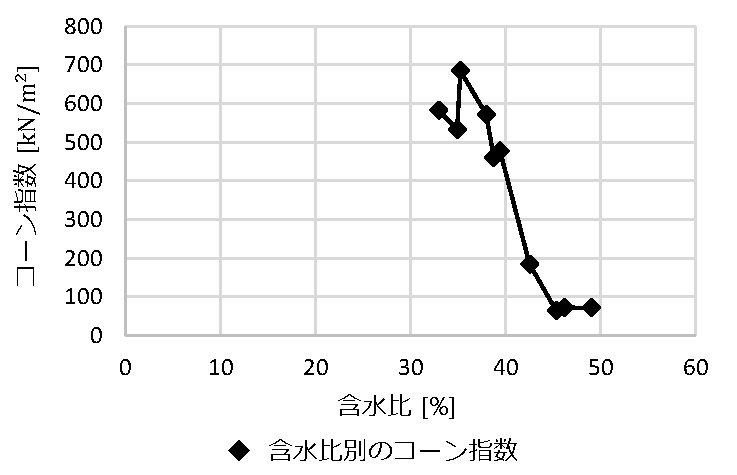
\includegraphics[width=11cm]{./ch5_ConeIndexEstimation/Fig/coneindex_and_watercontent_relationship_of_experimental_site_compressed}
            \caption{実験場所の土の含水比とコーン指数の関係}
            \label{fig:coneindex_and_watercontent_relationship_of_experimental_site}
      \end{center}
\end{figure}

\begin{figure}[p]
      \begin{center}
            \begin{tabular}{c}

                  \begin{minipage}[b]{\linewidth}
                  \centering
                  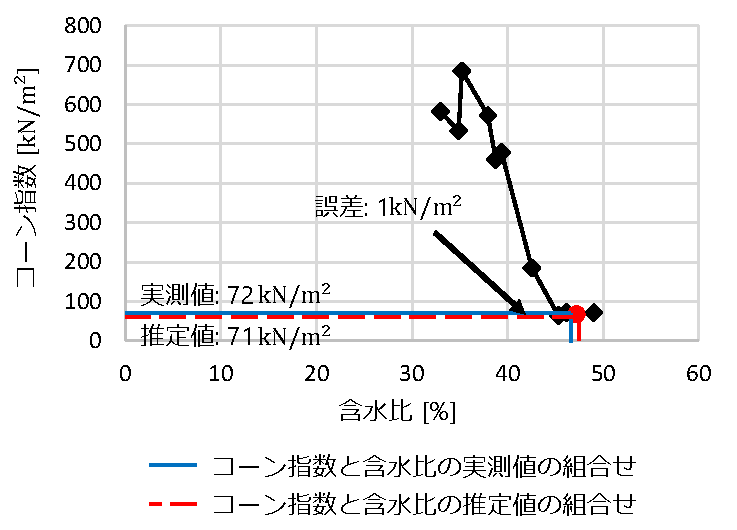
\includegraphics[width=11cm]{./ch5_ConeIndexEstimation/Fig/validationsoil_coneindex_and_watercontent_relationship_2ndrow_compressed.pdf}
                  \caption*{(a)表\ref{table.Calculated_cone_index}の上から2番目のコーン指数の実測値と推定値}
                  \end{minipage}

                  \\

                  \begin{minipage}[b]{\linewidth}
                  \centering
                  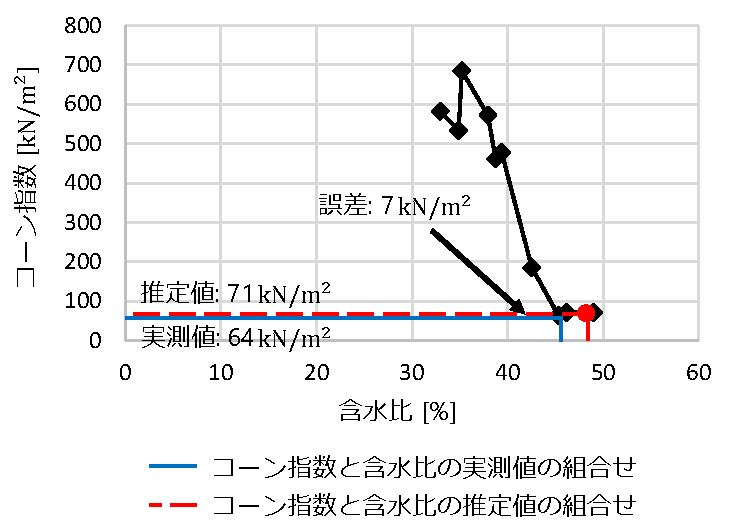
\includegraphics[width=11cm]{./ch5_ConeIndexEstimation/Fig/validationsoil_coneindex_and_watercontent_relationship_3rdrow_compressed.pdf}
                  \caption*{(b)表\ref{table.Calculated_cone_index}の上から3番目のコーン指数の実測値と推定値}
                  \end{minipage}

            \end{tabular}
      \caption{コーン指数の誤差が小さい場合}\label{fig:validationsoil_coneindex_and_watercontent_relationship_2ndrow_and_3rdrow}
      \end{center}
\end{figure}

\begin{figure}[p]
      \begin{center}
            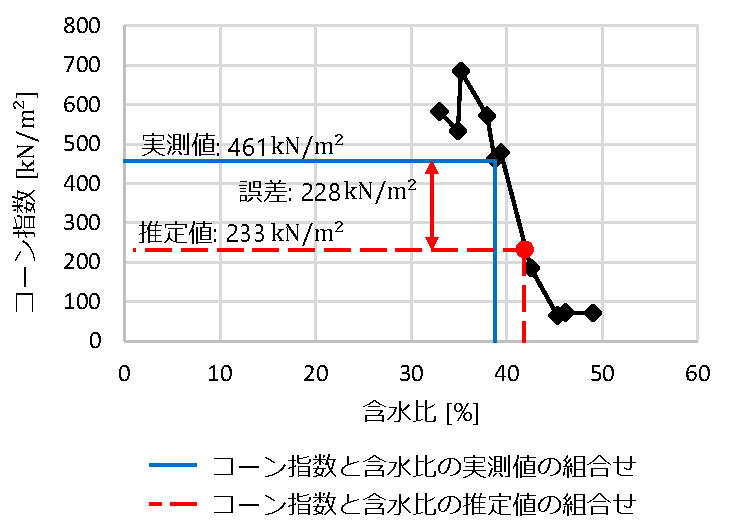
\includegraphics[width=11cm]{./ch5_ConeIndexEstimation/Fig/validationsoil_coneindex_and_watercontent_relationship_compressed.pdf}
            \caption{表\ref{table.Calculated_cone_index}の1番上のコーン指数の実測値と推定値}
            \label{fig:validationsoil_coneindex_and_watercontent_relationship}
      \end{center}
\end{figure}

\clearpage

\subsection{コーン指数に基づく走破性判定}
\label{ssec:TrafficabilityJudgementByConeindex}

履帯式の建設機械は,200${\rm kN/m^2}$以上のコーン指数の地盤を走破することができることが知られている\cite{古谷2016}.
そこで,マルチスペクトル画像を用いて推定したコーン指数に基づき,
コーン指数200${\rm kN/m^2}$を閾値として,走破性の判定を行い,
建設機械を実際に走破させた結果と比較した.
使用した建設機械は,コベルコ建機日本株式会社の油圧ショベルSK130UR-1Eである.
SK130UR-1Eは質量13400kg,全長7440mm,全幅2490mm,全高2730mmである.
SK130UR-1Eの外観を図\ref{fig:SK130UR-1E}に示す.
推定されたコーン指数が200${\rm kN/m^2}$以上の場合,走破可能であると判定し,
推定されたコーン指数が200${\rm kN/m^2}$未満の場合,走破困難であると判定した.
\ref{ssec:ConeindexEstimationExperimentResult}項で得られたコーン指数の推定値,およびその推定値から走破性を判定した結果を,
表\ref{table.trafficability_judgement_by_coneindex}に示す.
表\ref{table.trafficability_judgement_by_coneindex}において,
コーン指数の推定値が233${\rm kN/m^2}$となり200${\rm kN/m^2}$以上の場合は走破可能であると判定し,
コーン指数の推定値が71${\rm kN/m^2}$となり200${\rm kN/m^2}$未満の場合は走破困難であると判定した.

\begin{figure}[htbp]
      \begin{center}
            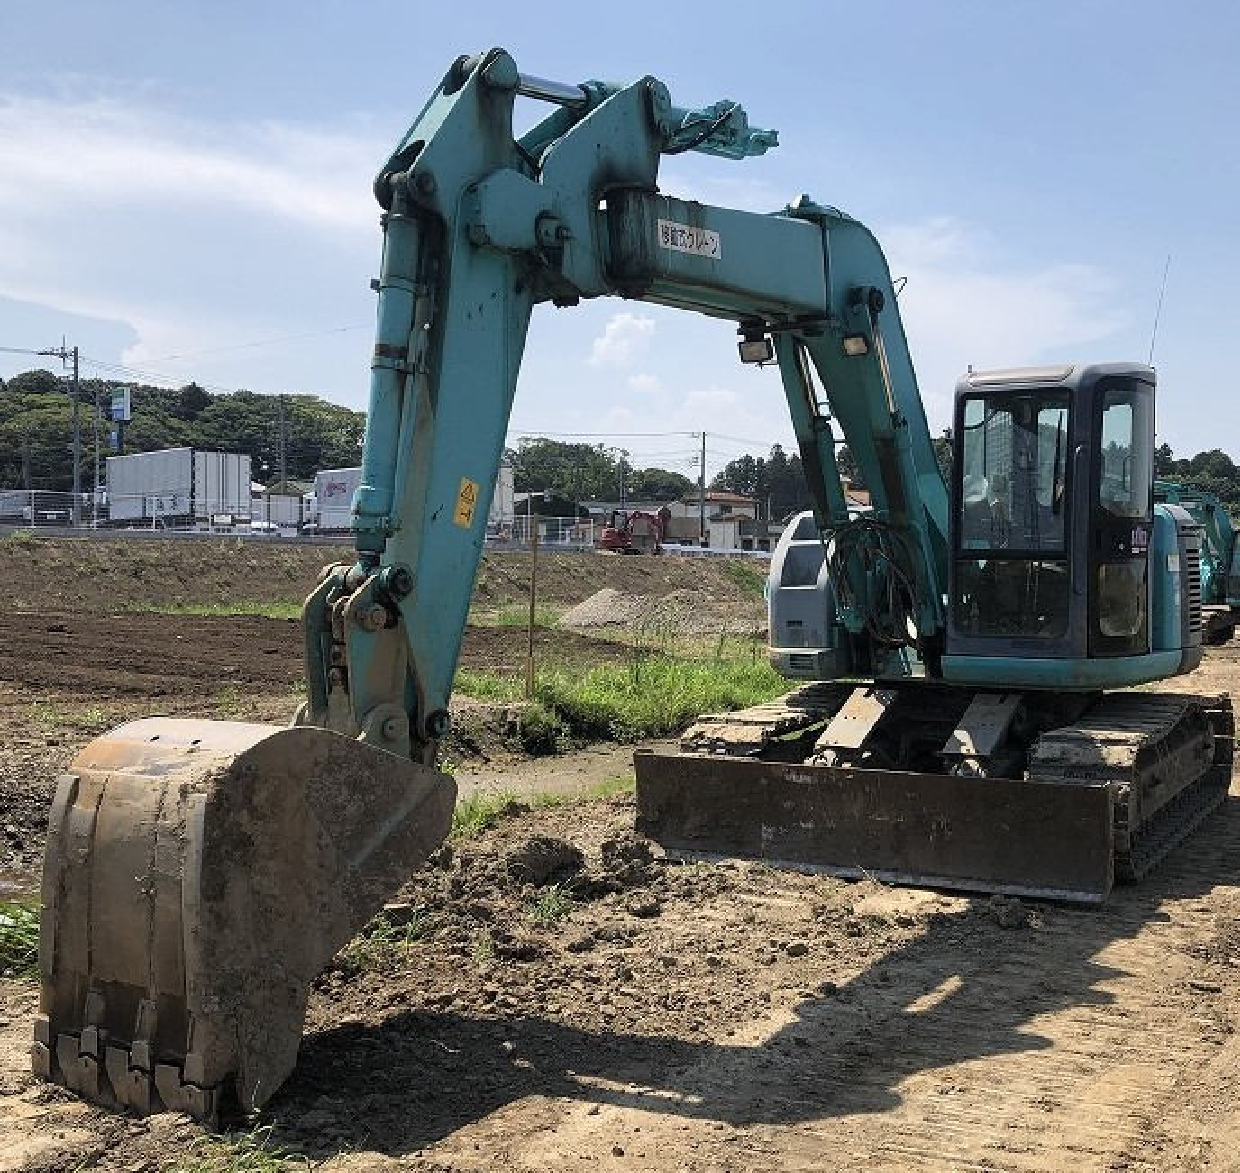
\includegraphics[width=5.5cm]{./ch5_ConeIndexEstimation/Fig/SK130UR-1E_compressed.pdf}
            \caption{走破性判定の確認に使用した油圧ショベルSK130UR-1E}
            \label{fig:SK130UR-1E}
      \end{center}
\end{figure}

\begin{table}[b]
      \begin{center}
            \caption{コーン指数の推定値に基づく走破性判定}
            \label{table.trafficability_judgement_by_coneindex}
            \begin{tabular}{|c|c|c|c|} \hline
            \textbf{\raisebox{-0.1em}{コーン指数の実測値}} \scalebox{0.85}{${\rm [kN/m^2]}$} & \raisebox{-0.1em}{461} & \raisebox{-0.1em}{72} & \raisebox{-0.1em}{64} \\ \hline
            \textbf{\raisebox{-0.1em}{コーン指数の推定値}} \scalebox{0.85}{${\rm [kN/m^2]}$} & \raisebox{-0.1em}{233} & \raisebox{-0.1em}{71} & \raisebox{-0.1em}{71} \\ \hline
            \textbf{\raisebox{-0.1em}{走破性判定}} & \raisebox{-0.1em}{可} & \multicolumn{2}{|c|}{\raisebox{-0.1em}{困難}} \\ \hline
            \end{tabular} 
      \end{center}
\end{table}

\clearpage

次に,表\ref{table.trafficability_judgement_by_coneindex}で示した走破性判定に対して,
建設機械を実際に走破させた結果を,図\ref{fig:validationsoil_trafficability_possible_coneindex_461_233}および図\ref{fig:trafficability_impossible}に示す.
図\ref{fig:validationsoil_trafficability_possible_coneindex_461_233}の画像は,
推定されたコーン指数に基づいて,走破可能であると判定された場合における建設機械の走破性を示す.
一方,図\ref{fig:trafficability_impossible}(a)および(b)の画像は,
推定されたコーン指数に基づいて,走破困難であると判定された場合における建設機械の走破性を示す.
図\ref{fig:validationsoil_trafficability_possible_coneindex_461_233}と図\ref{fig:trafficability_impossible}(a)および(b)の画像より,
推定されたコーン指数に基づく走破性判定と実際の走破性が一致していることが分かる.
コーン指数推定の検証実験で使用した土のコーン指数と含水比の関係は,図\ref{fig:coneindex_and_watercontent_relationship_of_experimental_site}に
示したように,コーン指数においては200${\rm kN/m^2}$周辺,そして含水比においては38$\%$から45$\%$の間で大きく変動する.
従って,この検証実験で使用した土においては,含水比が38$\%$未満,または45$\%$以上の場合は正確に走破性を判定できるが,
その中間領域では正確に判定できない可能性がある.

\begin{figure}[b]
      \begin{center}
            \begin{tabular}{c}

            \begin{minipage}[b]{\linewidth}
            \centering
            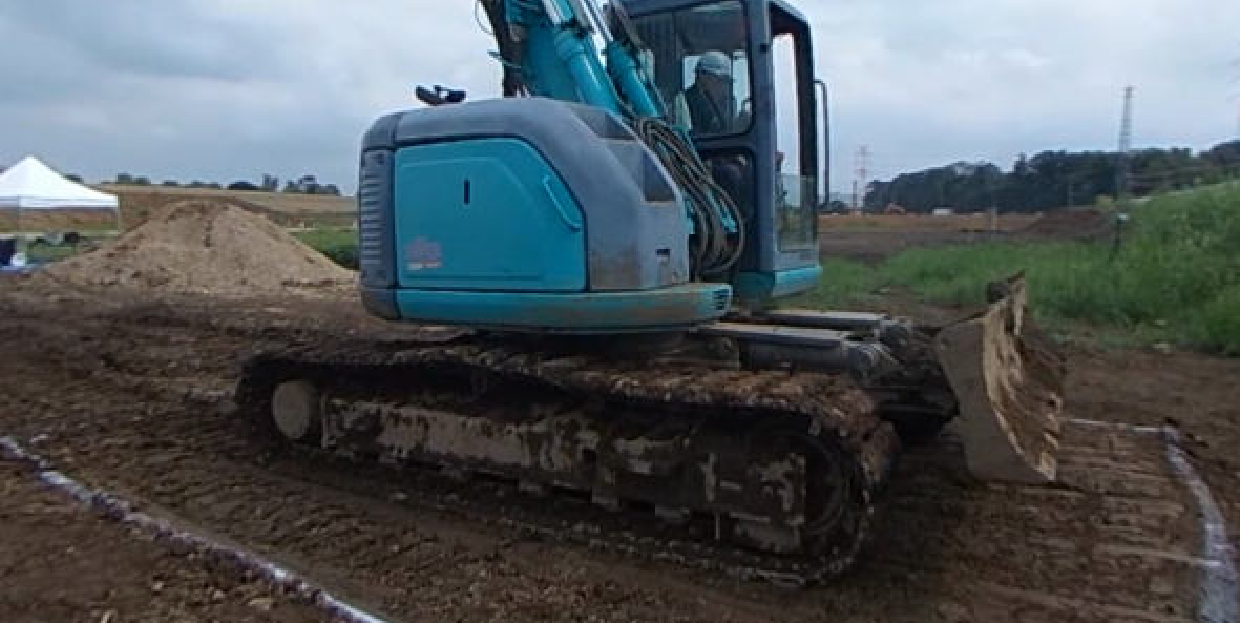
\includegraphics[width=12cm]{./ch5_ConeIndexEstimation/Fig/trafficability_coneindex_461_233_compressed.pdf}
            \setlength{\captionmargin}{50pt} % キャプションに使用する面積の両側の空白を調整
            \caption{走破可能であると判定された実験場所の実際の走破性\protect\linebreak(コーン指数の推定値: 71${\rm kN/m^2}$,コーン指数の実測値: 72${\rm kN/m^2}$)}
            \label{fig:validationsoil_trafficability_possible_coneindex_461_233}
            \vspace{3cm}
            \end{minipage}

            \end{tabular}
      \end{center}
\end{figure}

\begin{figure}[p]
      \begin{center}
            \begin{tabular}{c}

                  \begin{minipage}[b]{\linewidth}
                  \centering
                  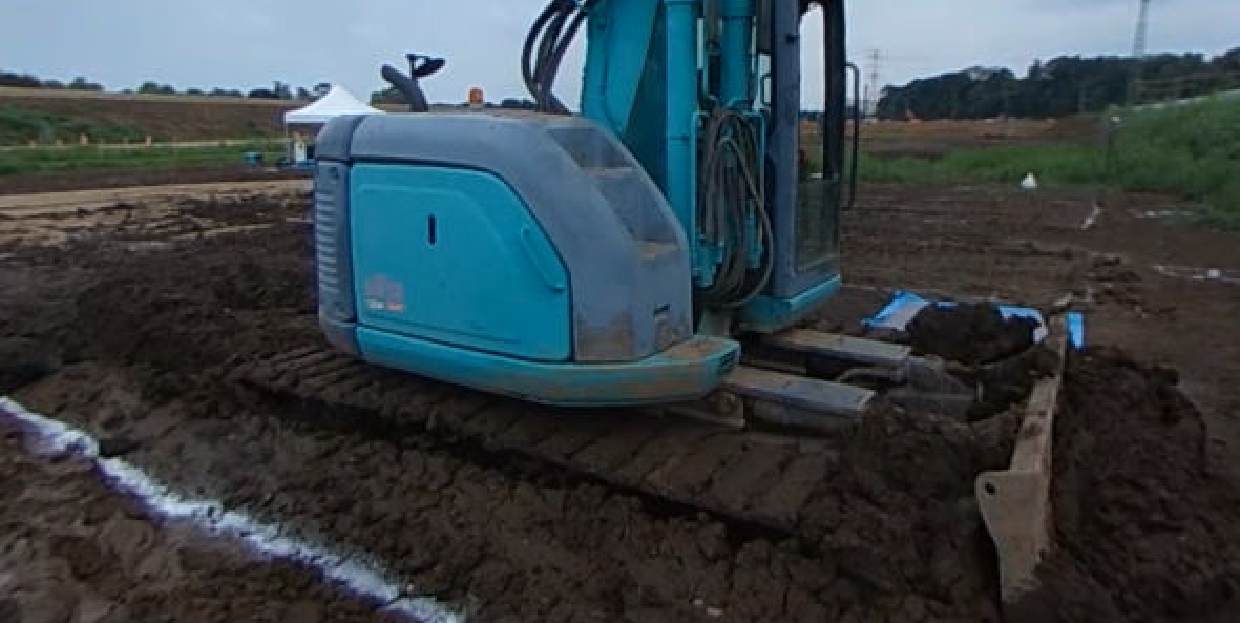
\includegraphics[width=12cm]{./ch5_ConeIndexEstimation/Fig/trafficability_coneindex_72_72_compressed.pdf}
                  \caption*{(a)コーン指数の推定値: 71${\rm kN/m^2}$,コーン指数の実測値: 72${\rm kN/m^2}$}
                  \vspace{1cm}
                  \end{minipage}

                  \\

                  \begin{minipage}[b]{\linewidth}
                  \centering
                  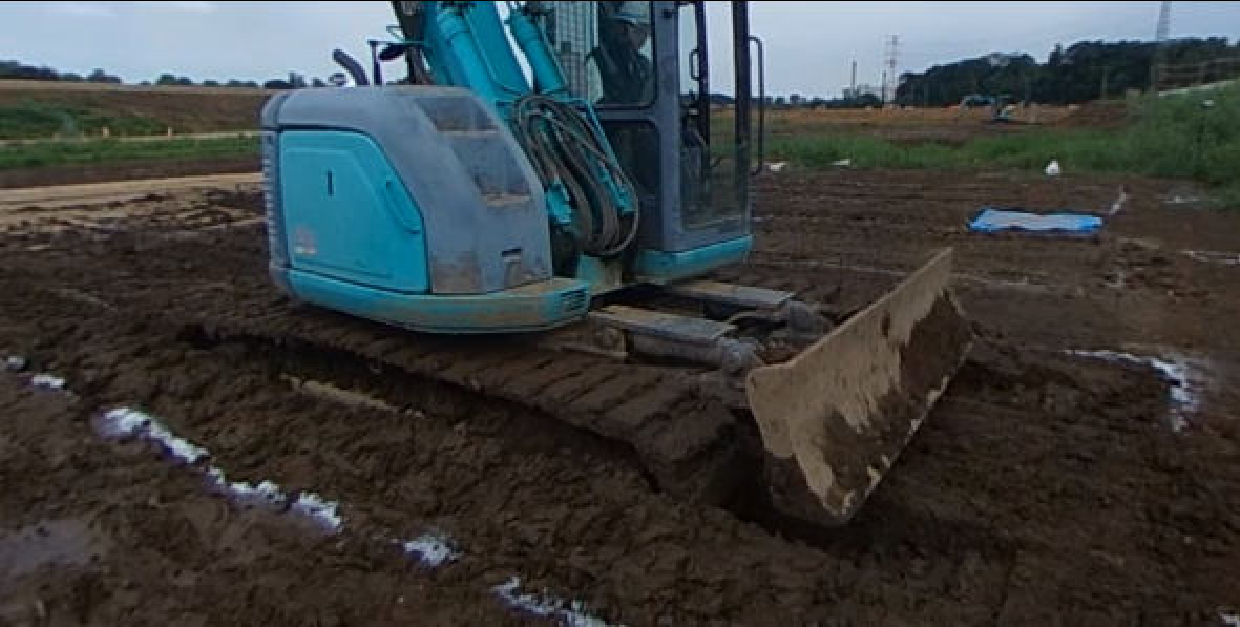
\includegraphics[width=12cm]{./ch5_ConeIndexEstimation/Fig/trafficability_coneindex_64_71_compressed.pdf}
                  \caption*{(b)コーン指数の推定値: 71${\rm kN/m^2}$,コーン指数の実測値: 64${\rm kN/m^2}$}
                  \end{minipage}

            \end{tabular}
      \caption{走破不可能であると判定された実験場所の実際の走破性}\label{fig:trafficability_impossible}
      \end{center}
\end{figure}

\clearpage

\subsection{考察}
\label{ssec:ConeindexEstimationExperimentConsideration}

\ref{ssec:ConeindexEstimationExperimentResult}項で示したコーン指数を推定する検証実験の結果より,
コーン指数推定の対象とする土の,
含水比に対するコーン指数の変動が穏やかな含水比の範囲においては,
含水比の実測値と推定値の存在する間でのコーン指数の変動が小さいので,
含水比の
誤差が数$\%$程度であれば,推定した含水比に基づいて推定したコーン指数と測定したコーン指数の誤差が非常に小さくなるため,
スペクトル画像を用いた非接触でのコーン指数の推定が可能であることが分かった.
一方,含水比に対するコーン指数の変動が激しい含水比の範囲においては,
含水比の実測値と推定値の存在する間でのコーン指数の変動が大きいので,
含水比の誤差が数$\%$程であっても,推定した含水比に基づいて推定したコーン指数と測定したコーン指数の誤差が大きくなるため,
スペクトル画像を用いた非接触でのコーン指数の推定が困難になることも分かった.

また,\ref{ssec:TrafficabilityJudgementByConeindex}項で示した走破性判定の結果より,
建設機械が走破できる限界と言われている200${\rm kN/m^2}$を閾値とすることによって,
推定したコーン指数に基づく非接触での走破性判定が可能であることが分かった.
しかし,上記で解説したように,コーン指数の推定値と測定したコーン指数の誤差が大きくなる場合には,
走破性判定が困難になる.

\clearpage


%==============================================================================
%おわりに
%==============================================================================
\section{おわりに}

本章では,第\ref{ch:SoilTypeDiscrimination}章で識別した土の種類と,
第\ref{ch:WaterContentEstimation}章で推定した含水比を用いて,
コーン指数を推定する手法について述べた.

まず,\ref{sec:InfluenceOfSoilTypeAndWaterContentToConeIndex}節において,
土の粒子の鉱物組成,有機物含有量,粒度分布,球形率が同じ土を同じ種類であると定義した土の種類を,取得する波長帯の数が非常に多いマルチスペクトル画像から
識別し,含水比を,取得する波長帯の数が少ないマルチスペクトル画像から推定することによって,非接触でコーン指数を推定することを述べた.

次に,\ref{sec:ConeIndexEstimation}節において,
土の種類ごとに異なる含水比とコーン指数の関係を記録することによって,
土の種類と含水比からコーン指数を推定することを述べた.

最後に,\ref{sec:ConeindexEstimationExperiment}節において,
屋外で行ったコーン指数推定の検証実験の詳細を述べた.
検証実験において推定したコーン指数と測定したコーン指数を比較した結果,
コーン指数を推定する土の,含水比に対するコーン指数の変動が穏やかな含水比の範囲においては,
スペクトル画像を用いた非接触でのコーン指数の推定と,推定したコーン指数に基づく非接触での走破性判定が
可能であることが分かった.

\newpage
%%%%%%%%%%%%%%%%%%%%%%%%%%%%%%%%%%%%%%%%%%%%%%%%%%%%%%%%%%%%%%%%%%%%%%%%%%%%%%%